\section[Factoring Out Symmetries in Two--Dimensional~Images]{Factoring Out Symmetries in Two--Dimensional~Images}

\begin{frame}{Images Instead of Concentration Profiles}
	
	\centering
    As a preprocessing step, we have to take fluorescent images of the embryo~cross-sections and convert them to concentration profiles on a ring.
    
    \centering
    \begin{tikzpicture}
        \node (dpERKimage) {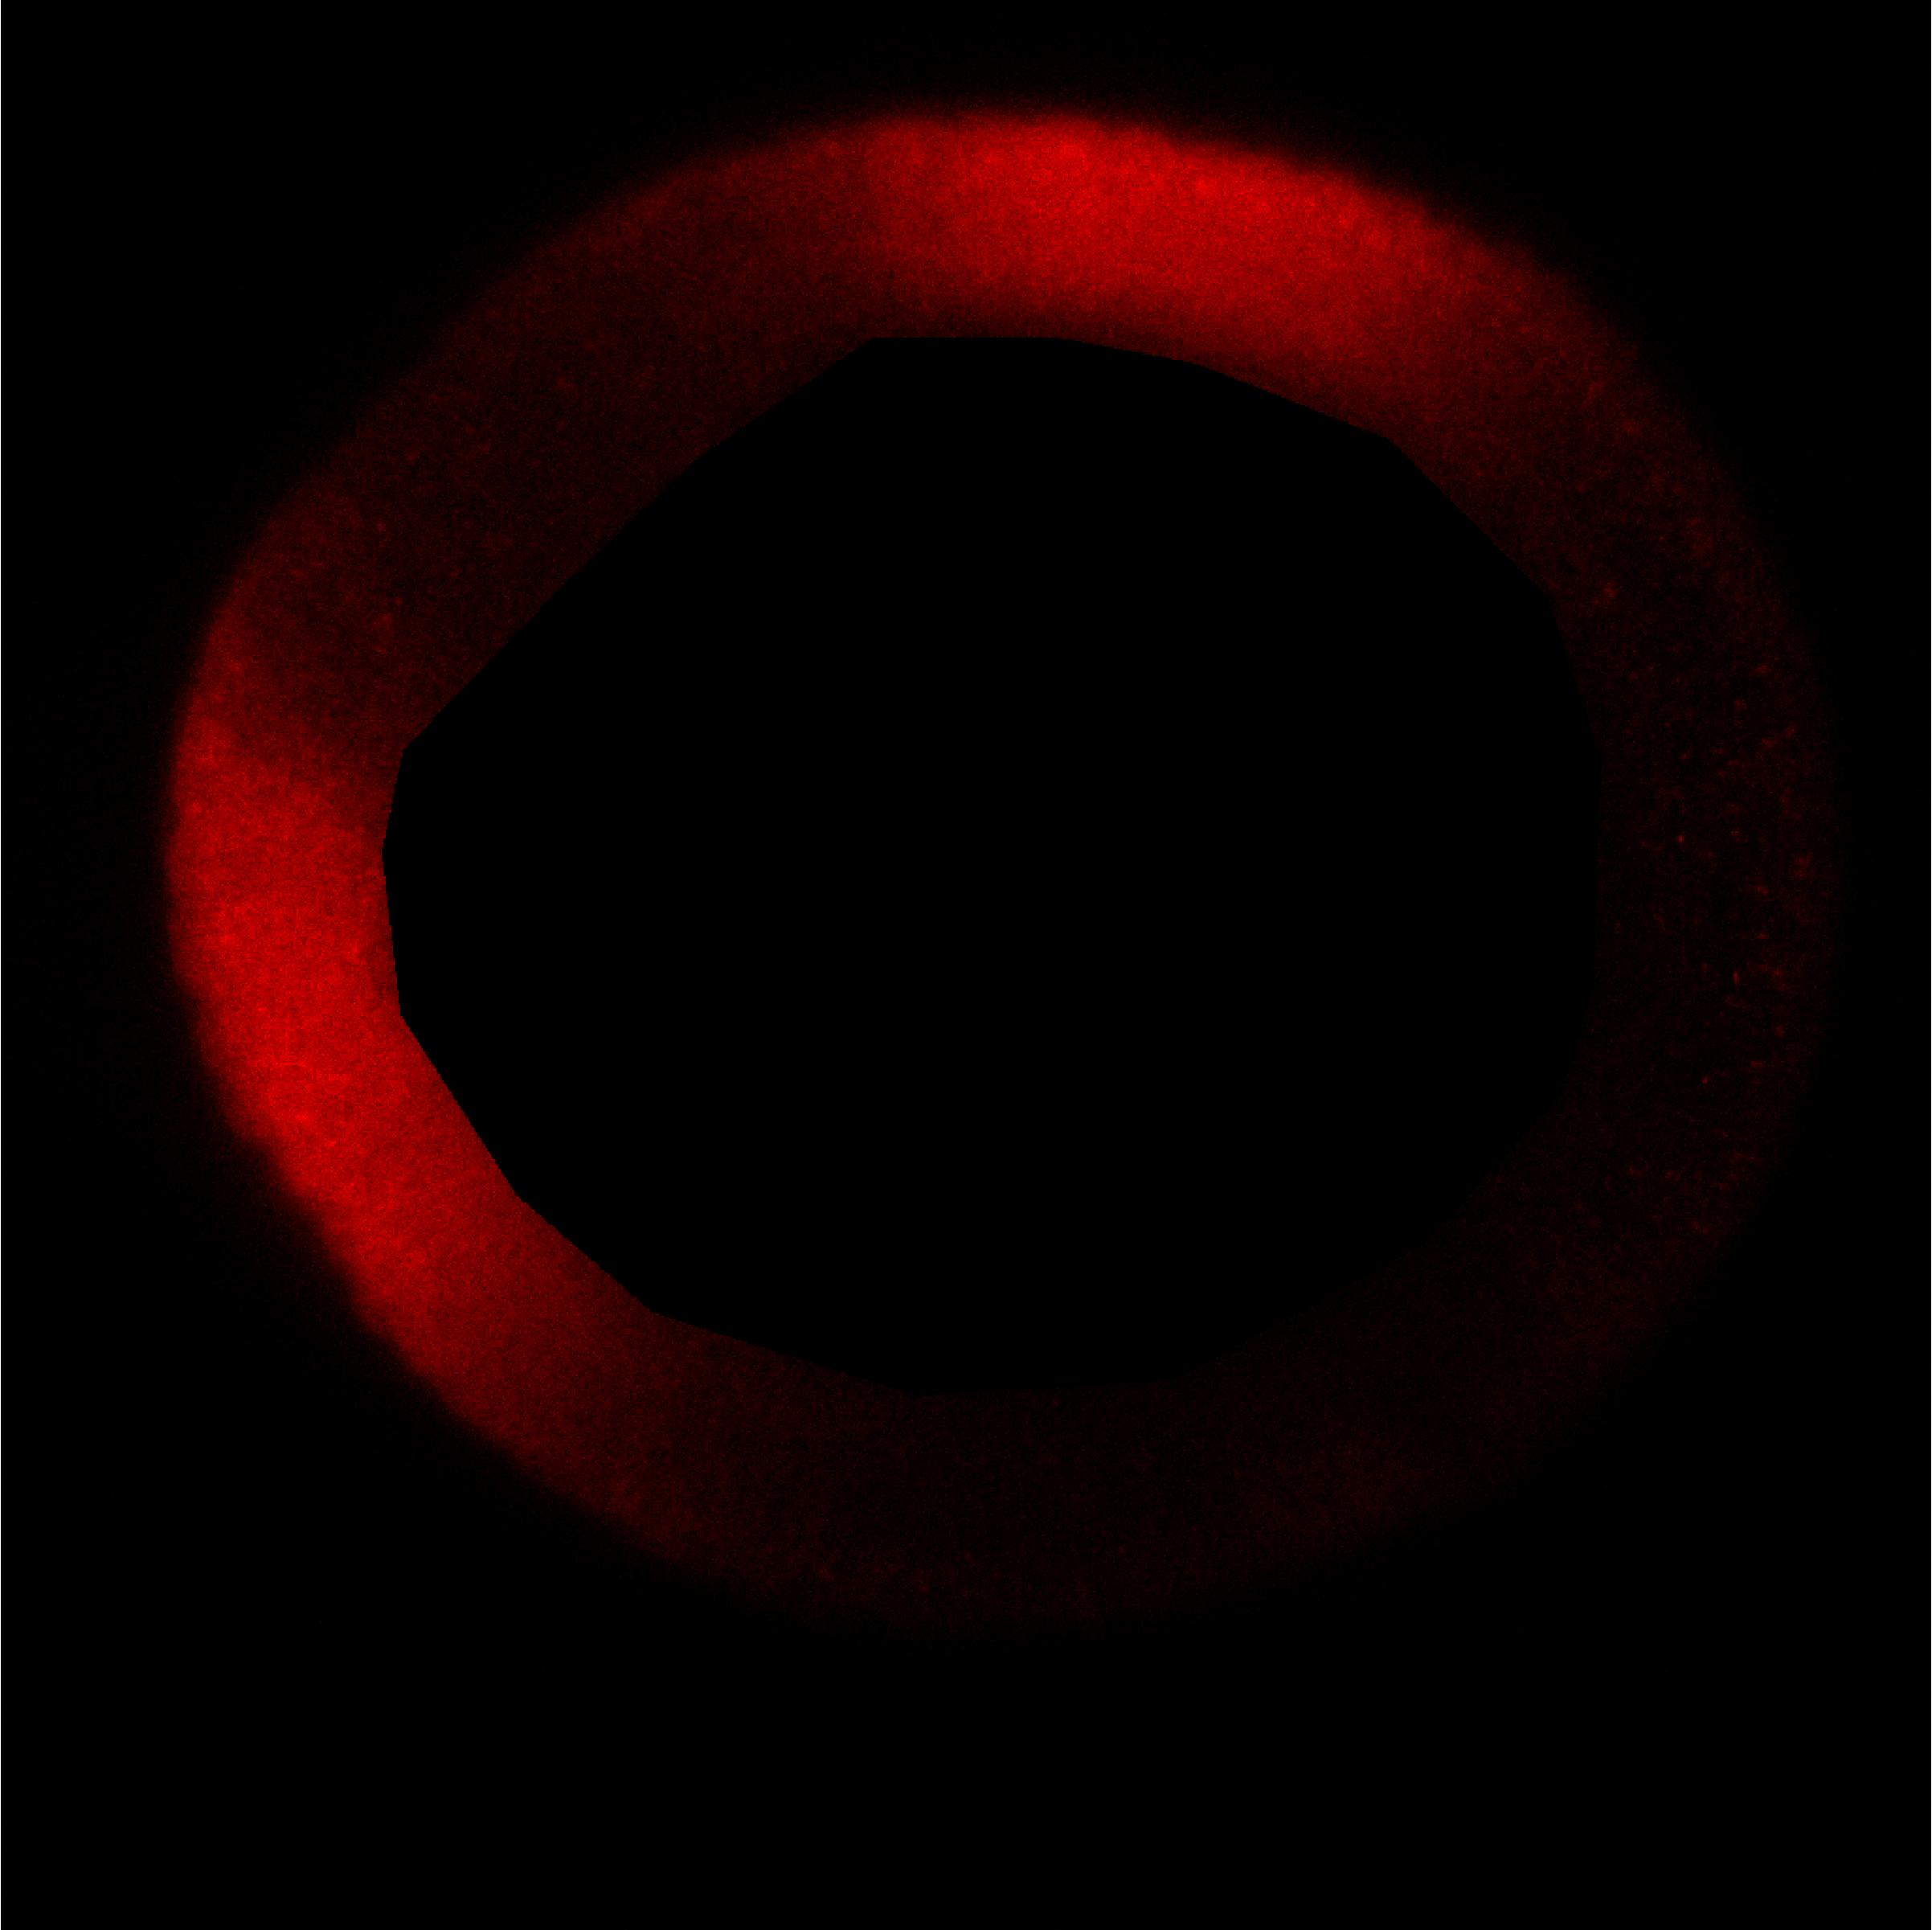
\includegraphics[width=0.3\textwidth]{drosophila_dpERK}};
        		\draw[gray,<->] (dpERKimage.south west) --  (dpERKimage.south east) node[below,midway] { \tiny $100 \mu m$};

        \node[right=of dpERKimage] (dpERKprofile) {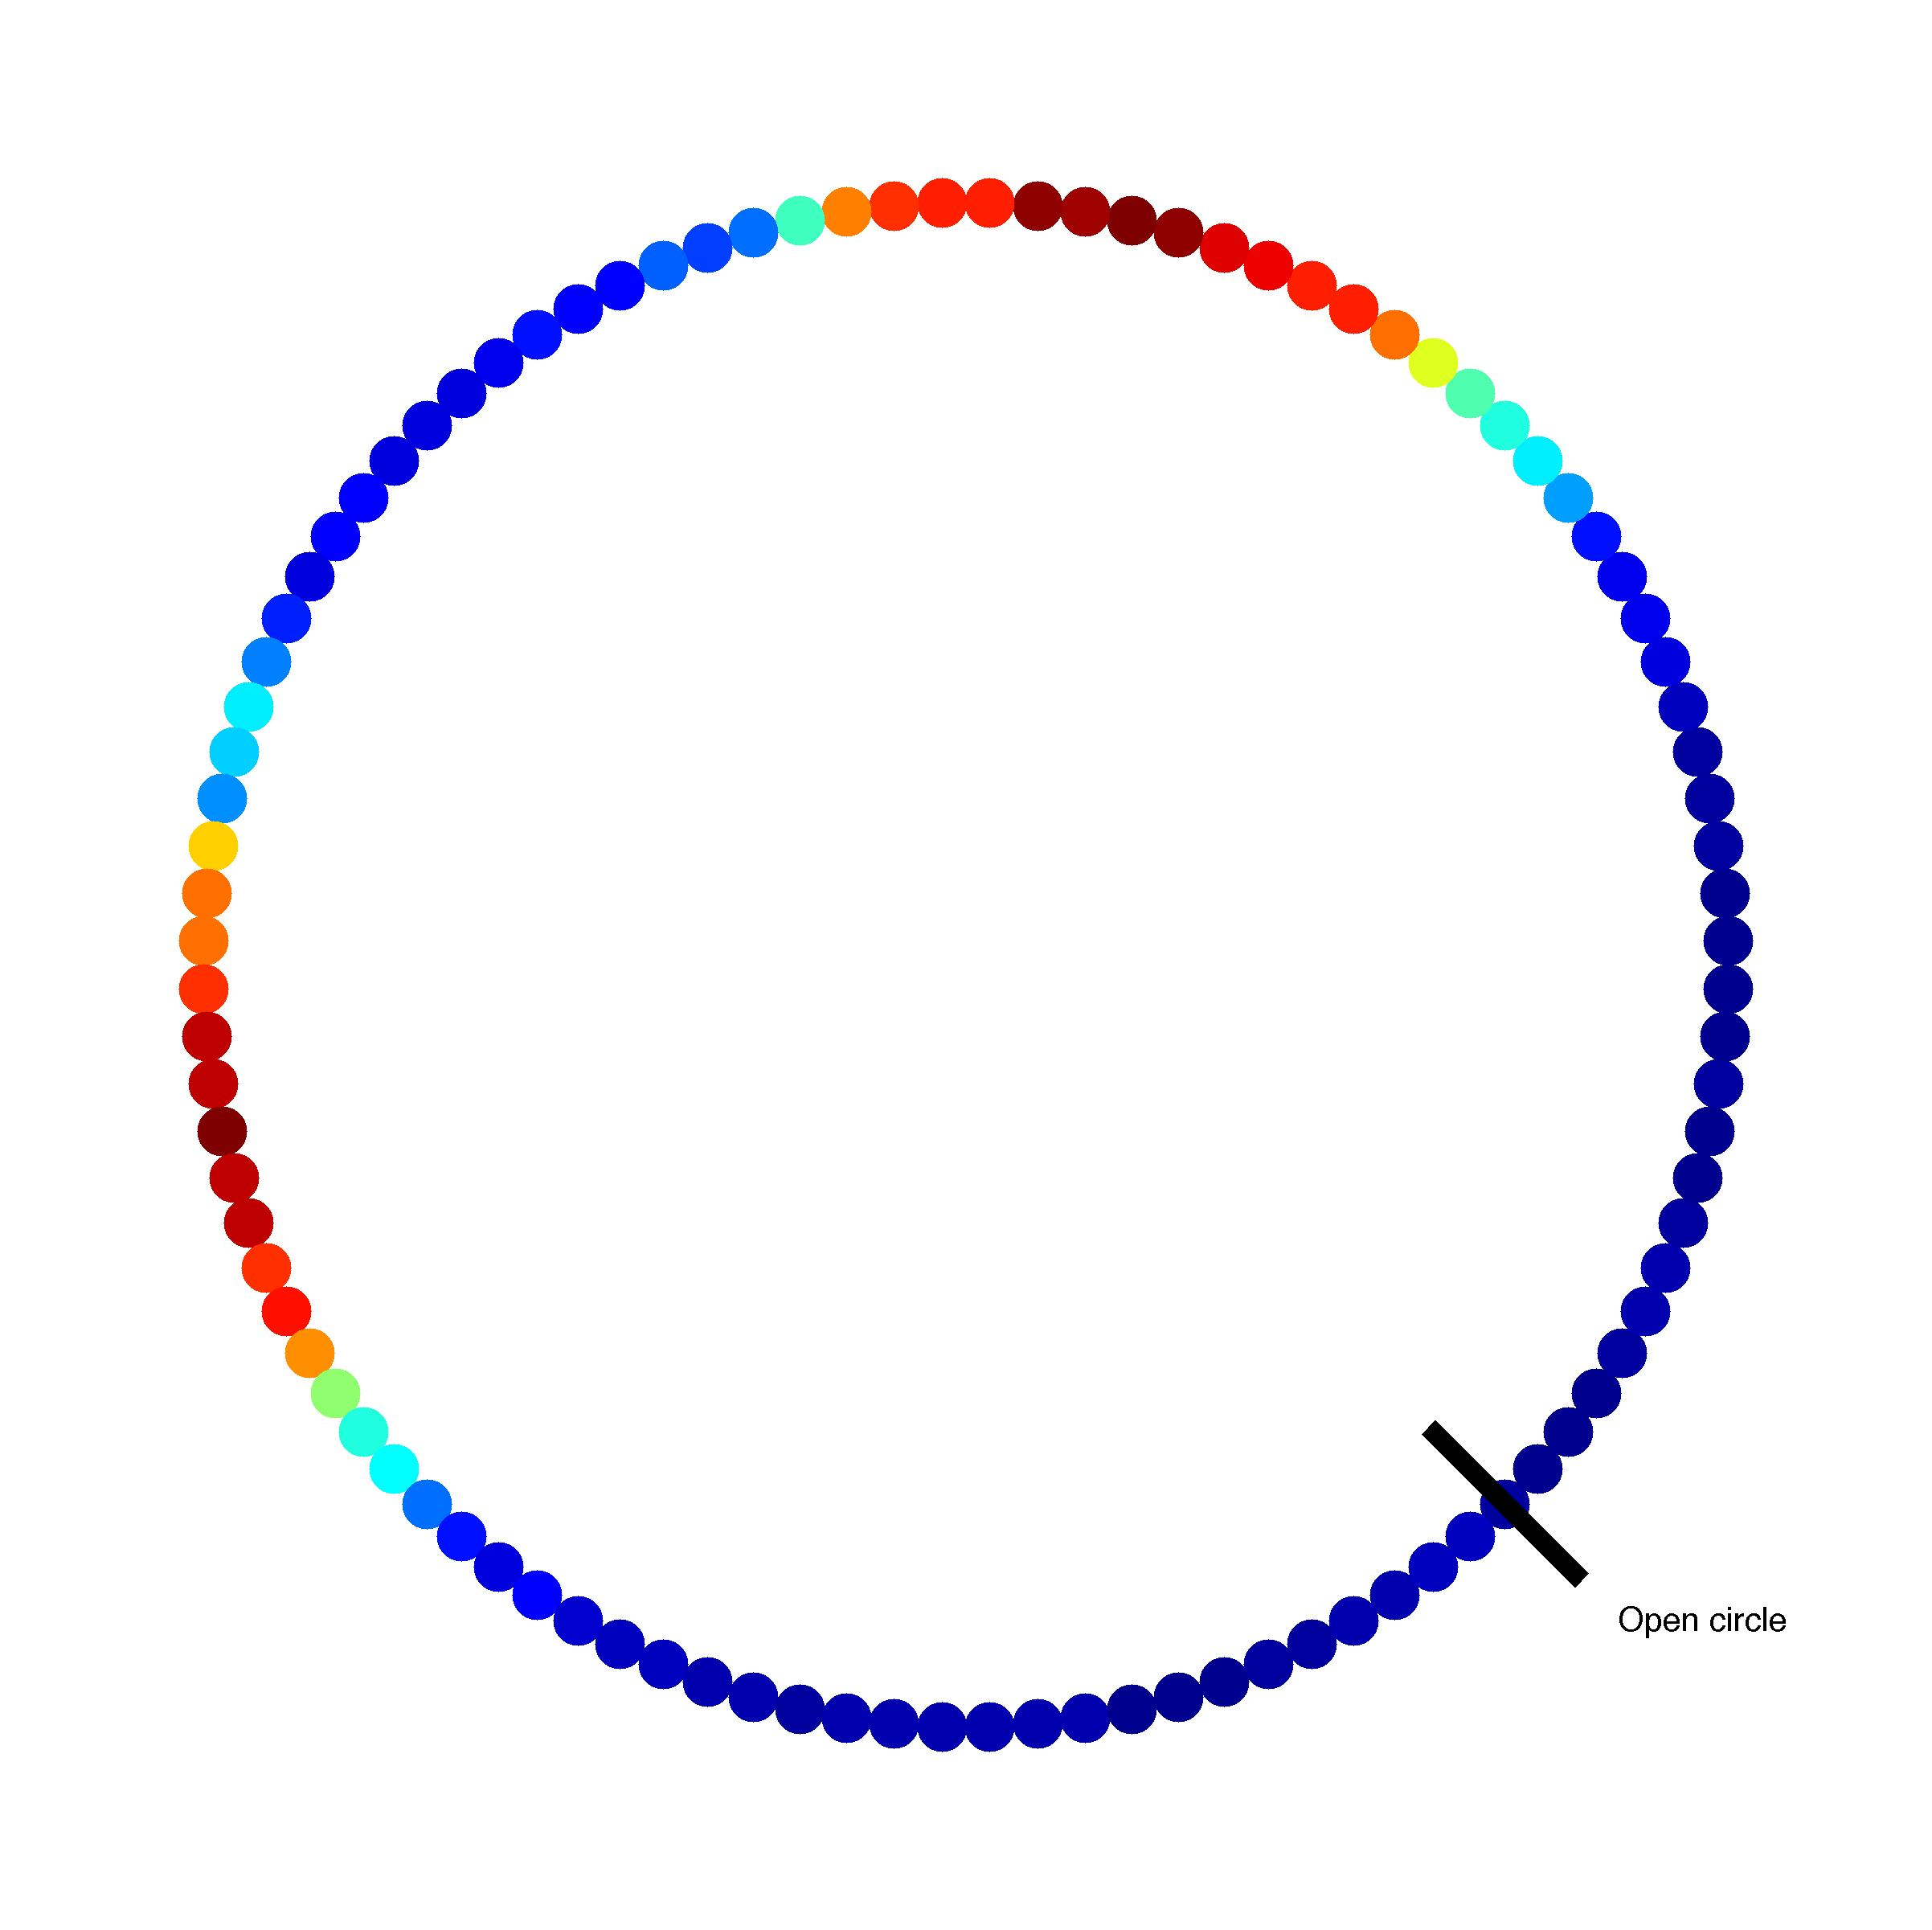
\includegraphics[width=0.3\textwidth]{circle_profile}};
        \draw[->] (dpERKimage)--(dpERKprofile);
    \end{tikzpicture}
    
    However, we could do the same analysis with {\bf raw images} instead of the concentration profiles to extract the dynamics.
    
    We must now synchronize/align the images under all {\bf translations and rotations}.
    
	\end{frame}

\begin{frame}{Alignment of Two-Dimensional Images}
    We align and order the images using vector diffusion maps.\\
    The VDM embedding coordinate is well-correlated with the membrane thickness.
    
    \centering
    \begin{tikzpicture}
    	\node[anchor=south west] (image) {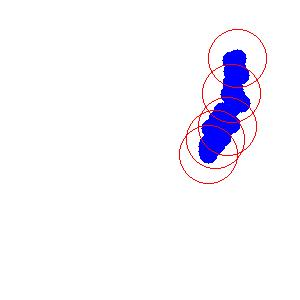
\includegraphics[width=0.5\textwidth]{vdm_2d_time_corr2}};
    	\begin{scope}[x={(image.south east)},y={(image.north west)}]
    	%\draw[help lines,xstep=.05,ystep=.05] (0,0) grid (1,1);
    	\node(x1) at (0.23,0.18) {};
    	\node(x2) at (0.34,0.27) {};
    	\node(x3) at (0.52,0.37) {};
    	\node(x4) at (0.58,0.58) {};
    	\node(x5) at (0.67,0.81) {};
    	\end{scope}
    	\node[below=0.2in of image](fig3) {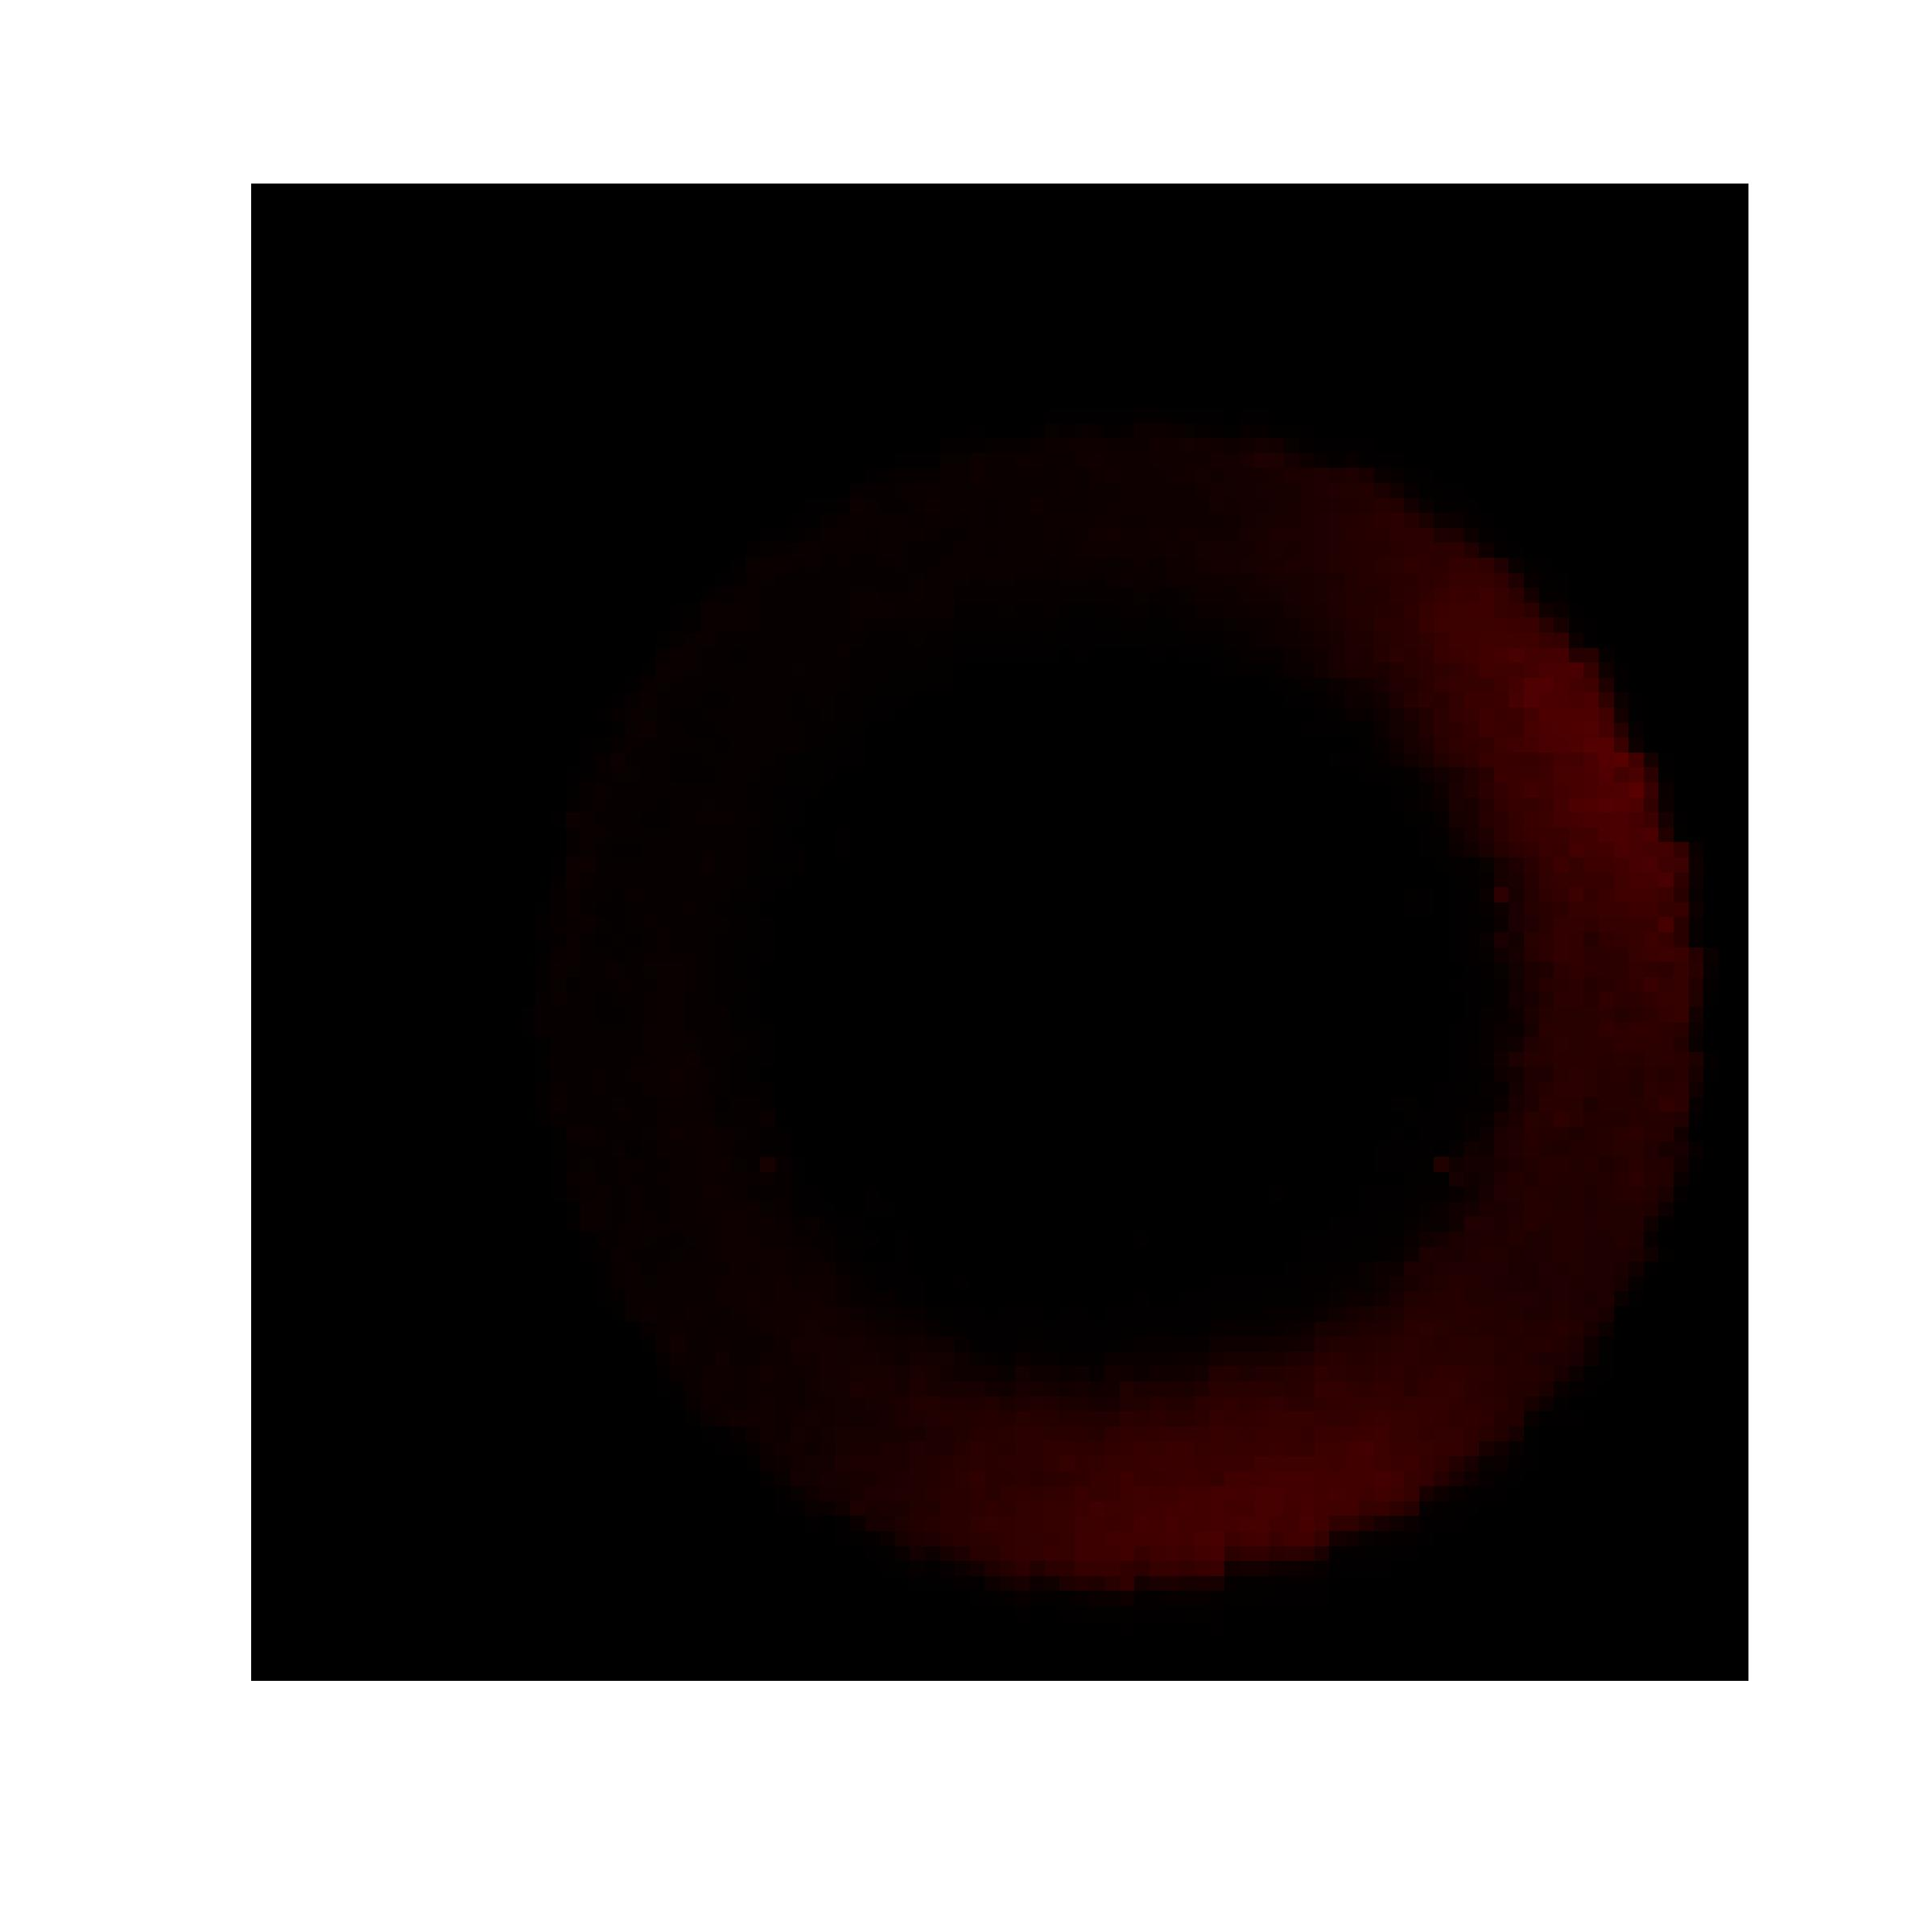
\includegraphics[width=0.1\textwidth]{dpERK_vdm_3}};		
    	\node[left=0.1in of fig3](fig2) {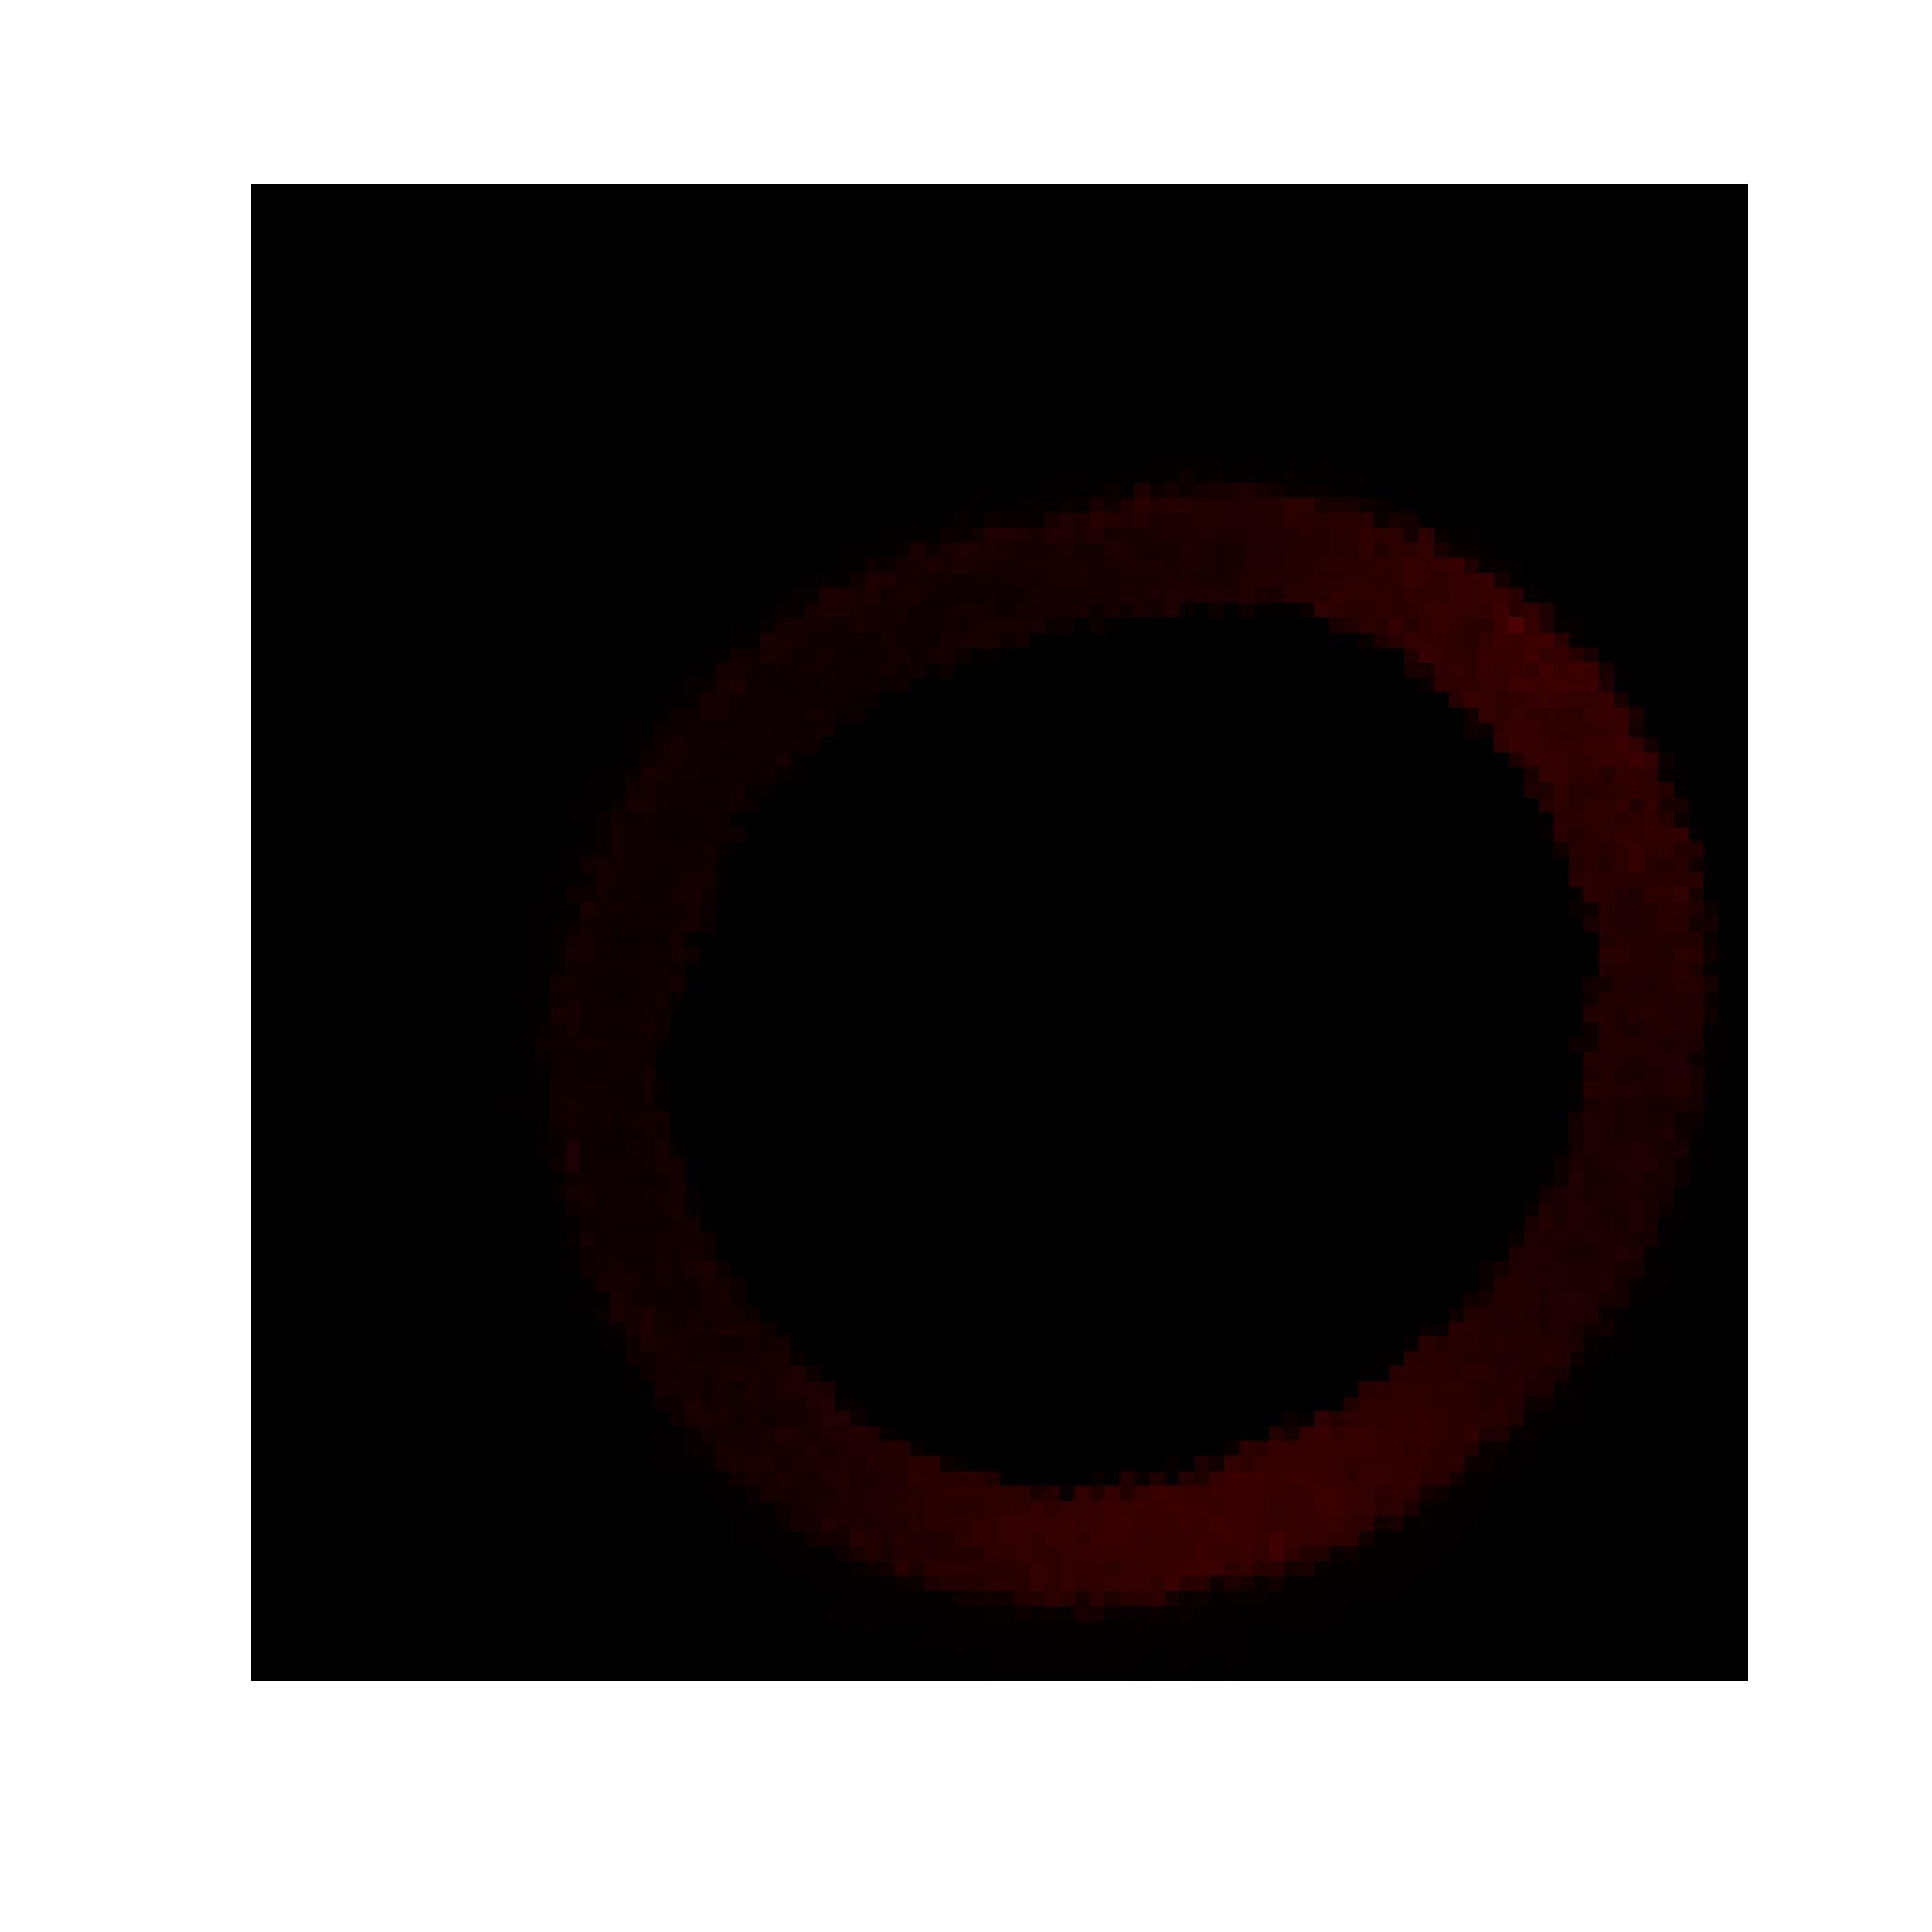
\includegraphics[width=0.1\textwidth]{dpERK_vdm_2}};
    	\node[left=0.1in of fig2](fig1) {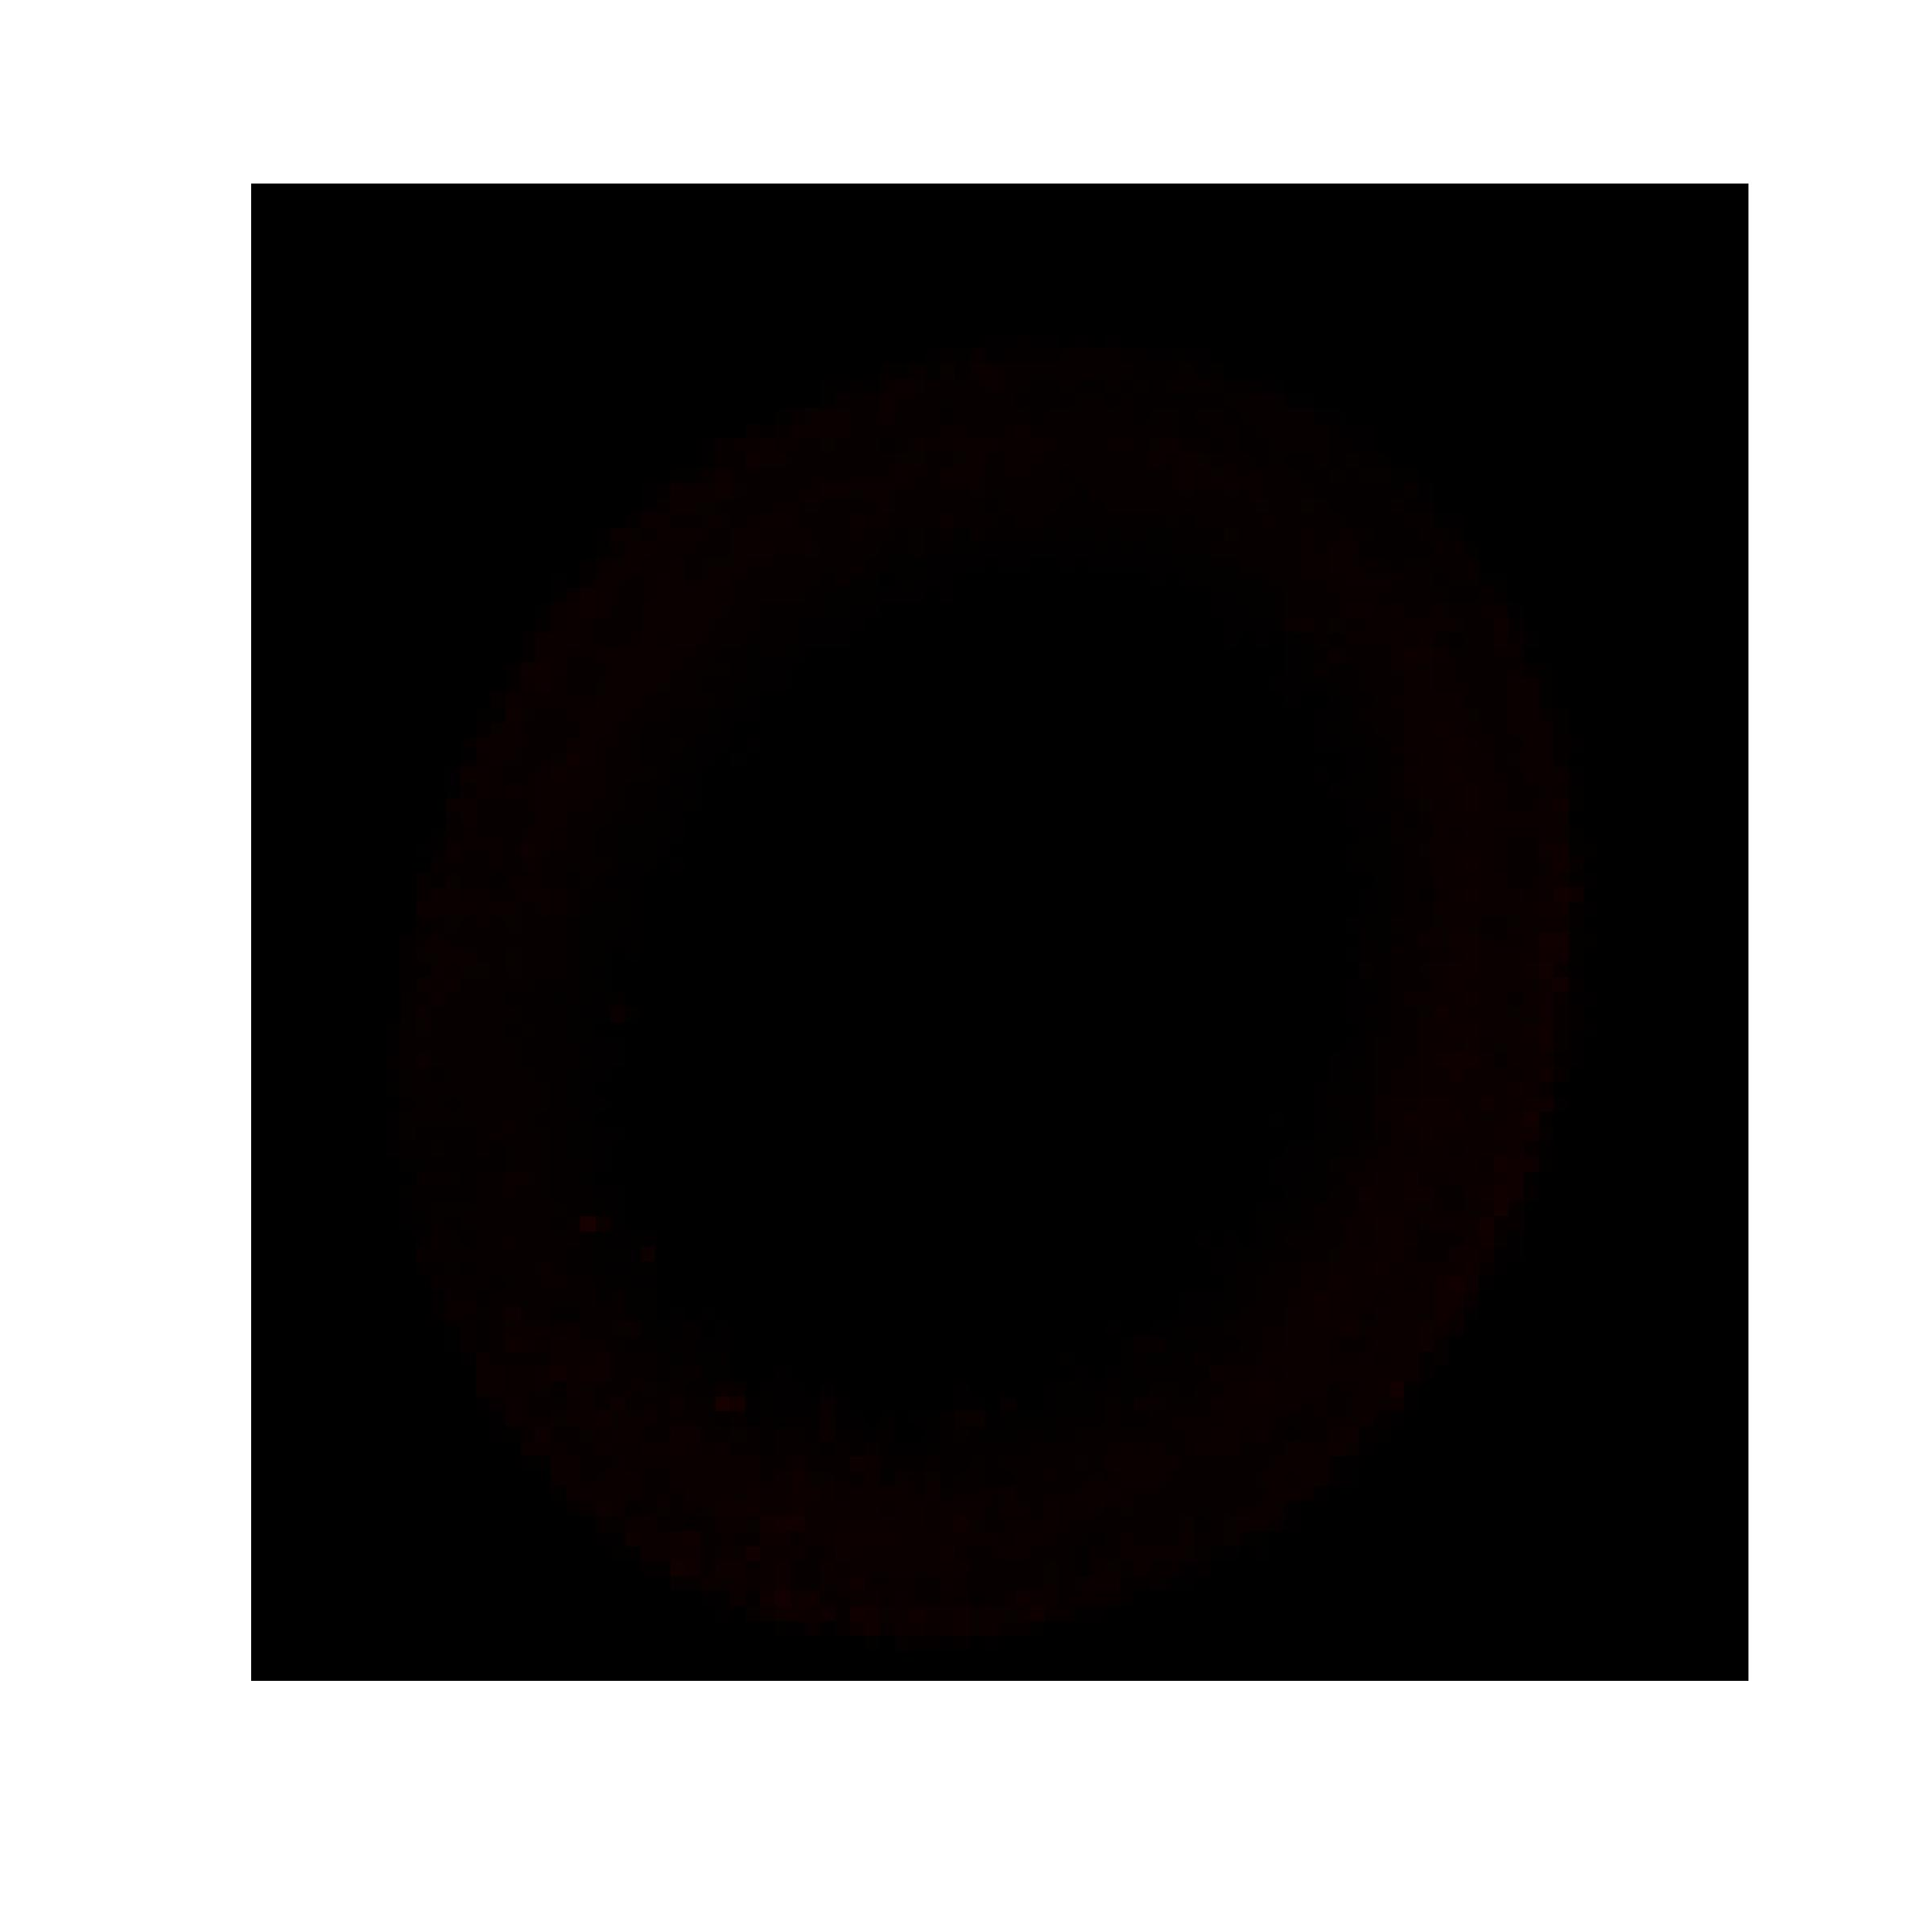
\includegraphics[width=0.1\textwidth]{dpERK_vdm_1}};	
    	\node[right=0.1in of fig3](fig4) {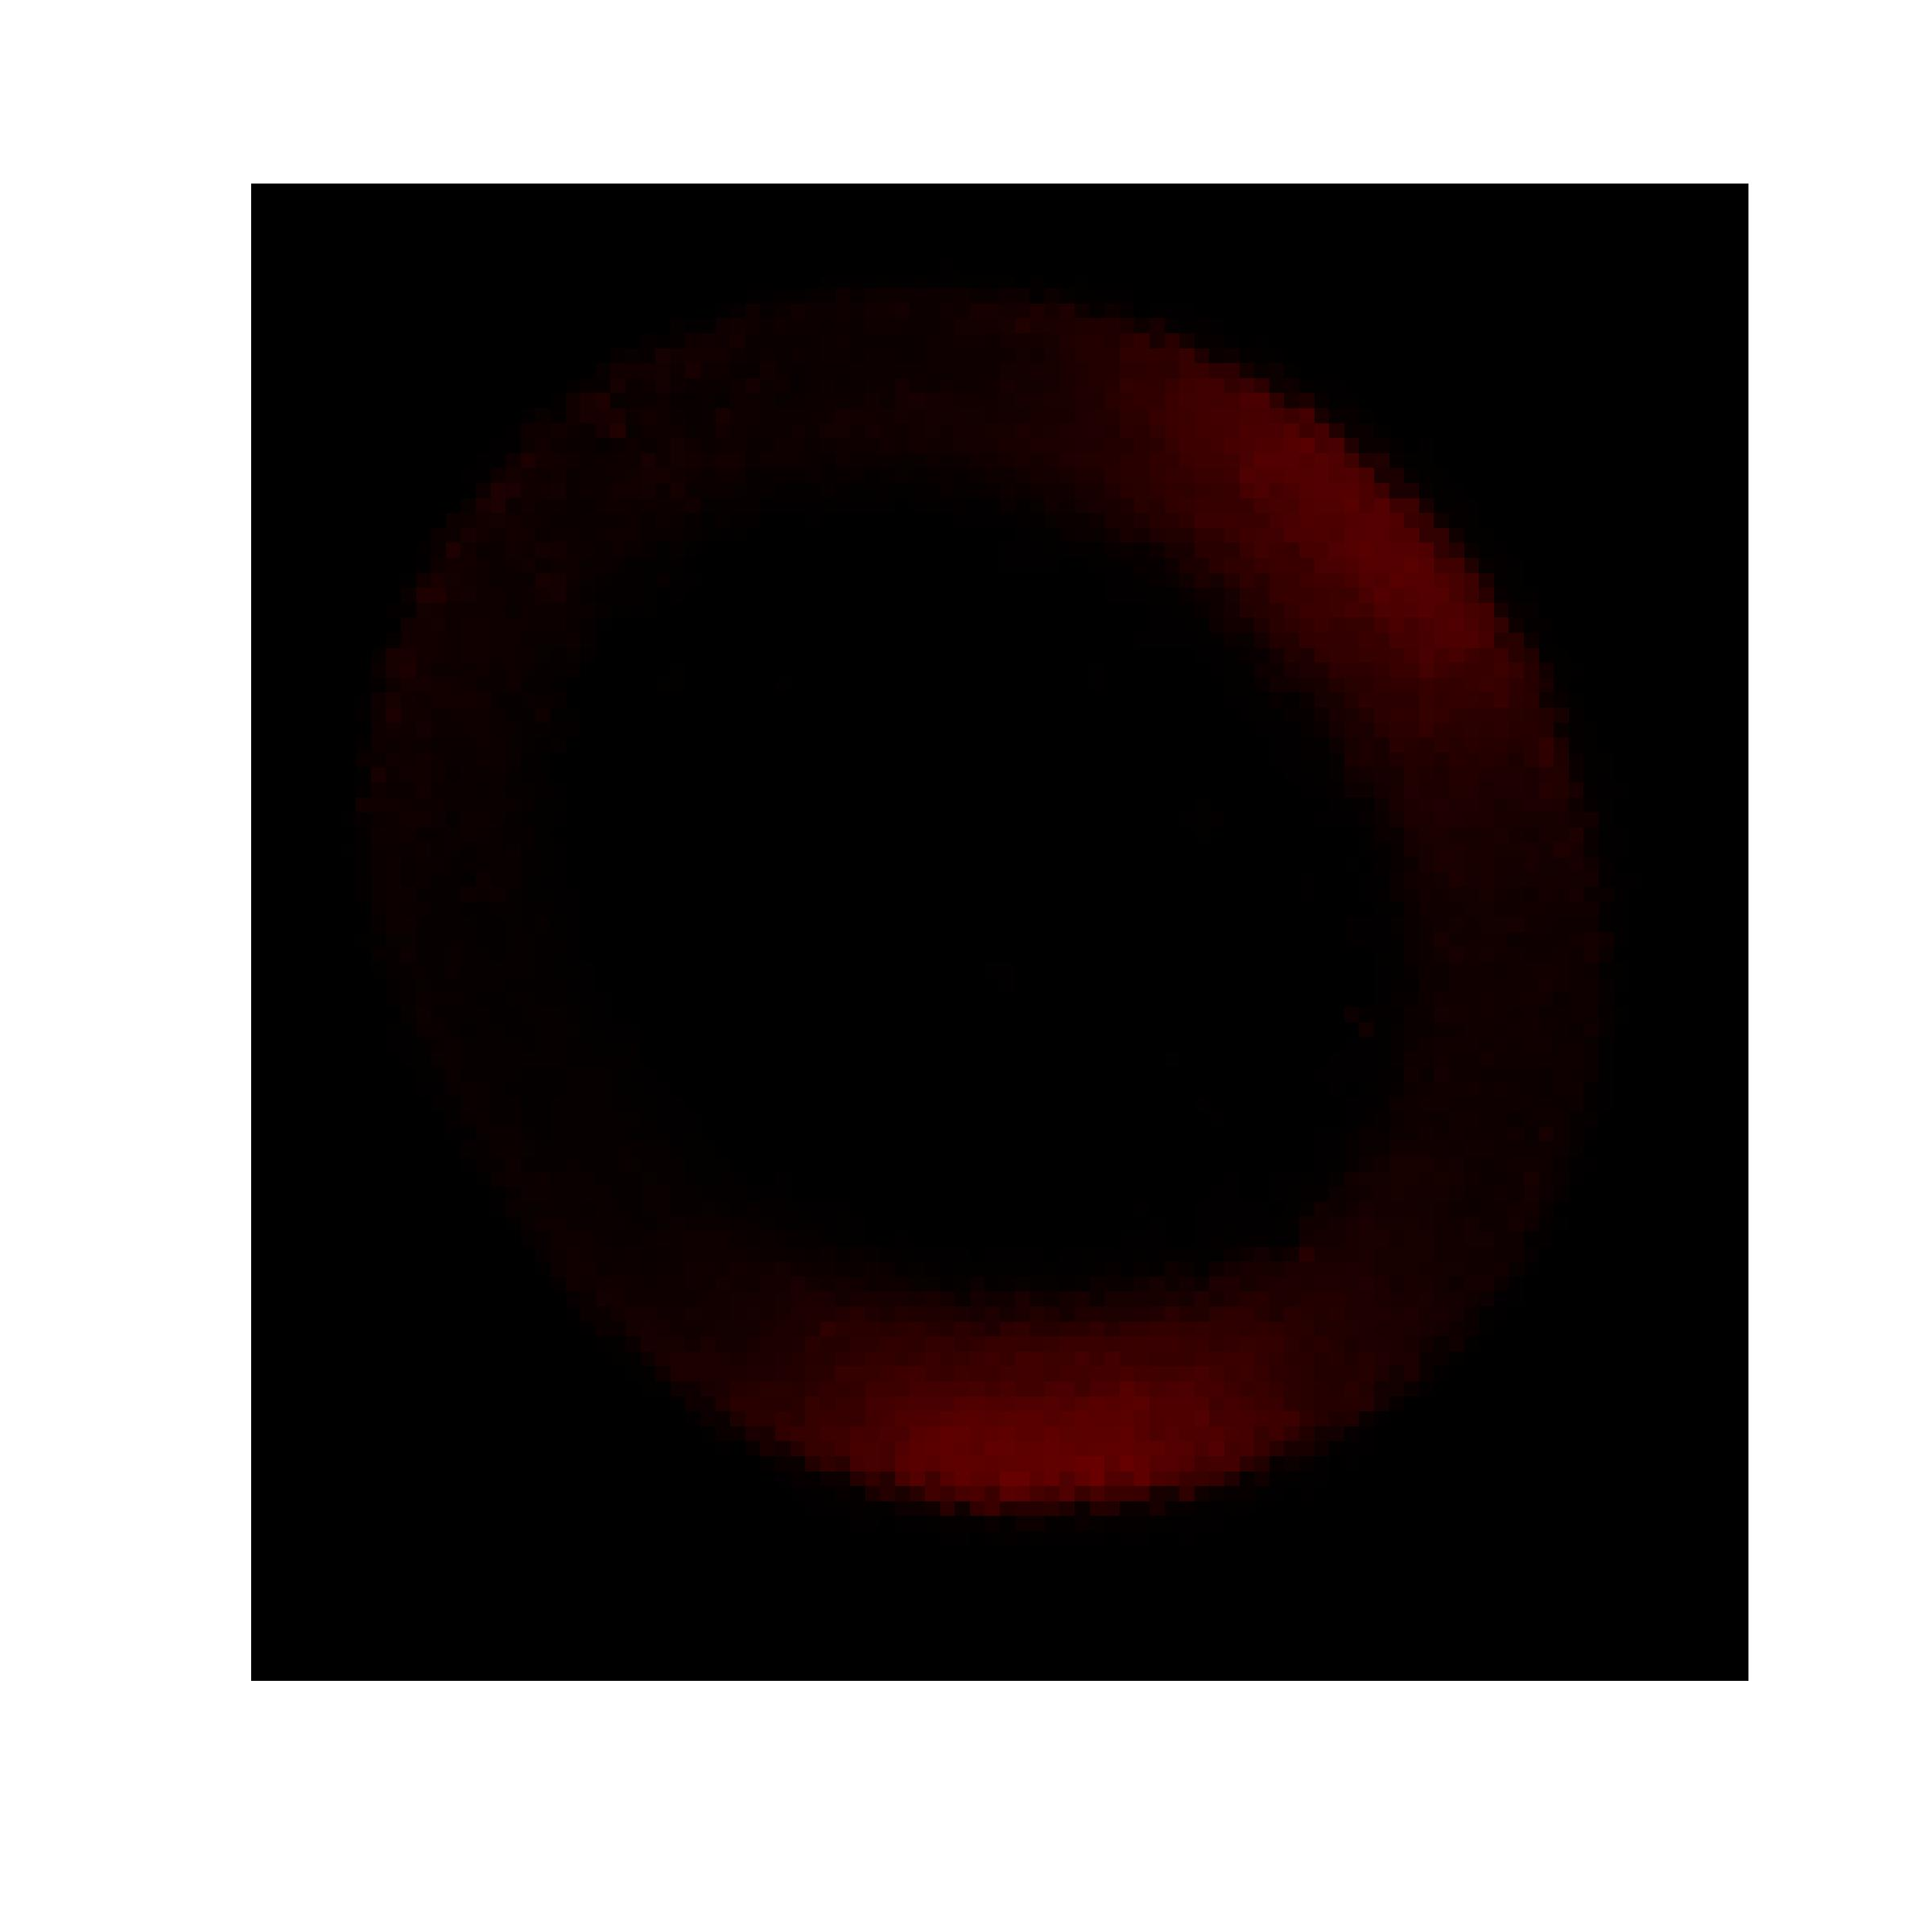
\includegraphics[width=0.1\textwidth]{dpERK_vdm_4}};					
    	\node[right=0.1in of fig4](fig5) {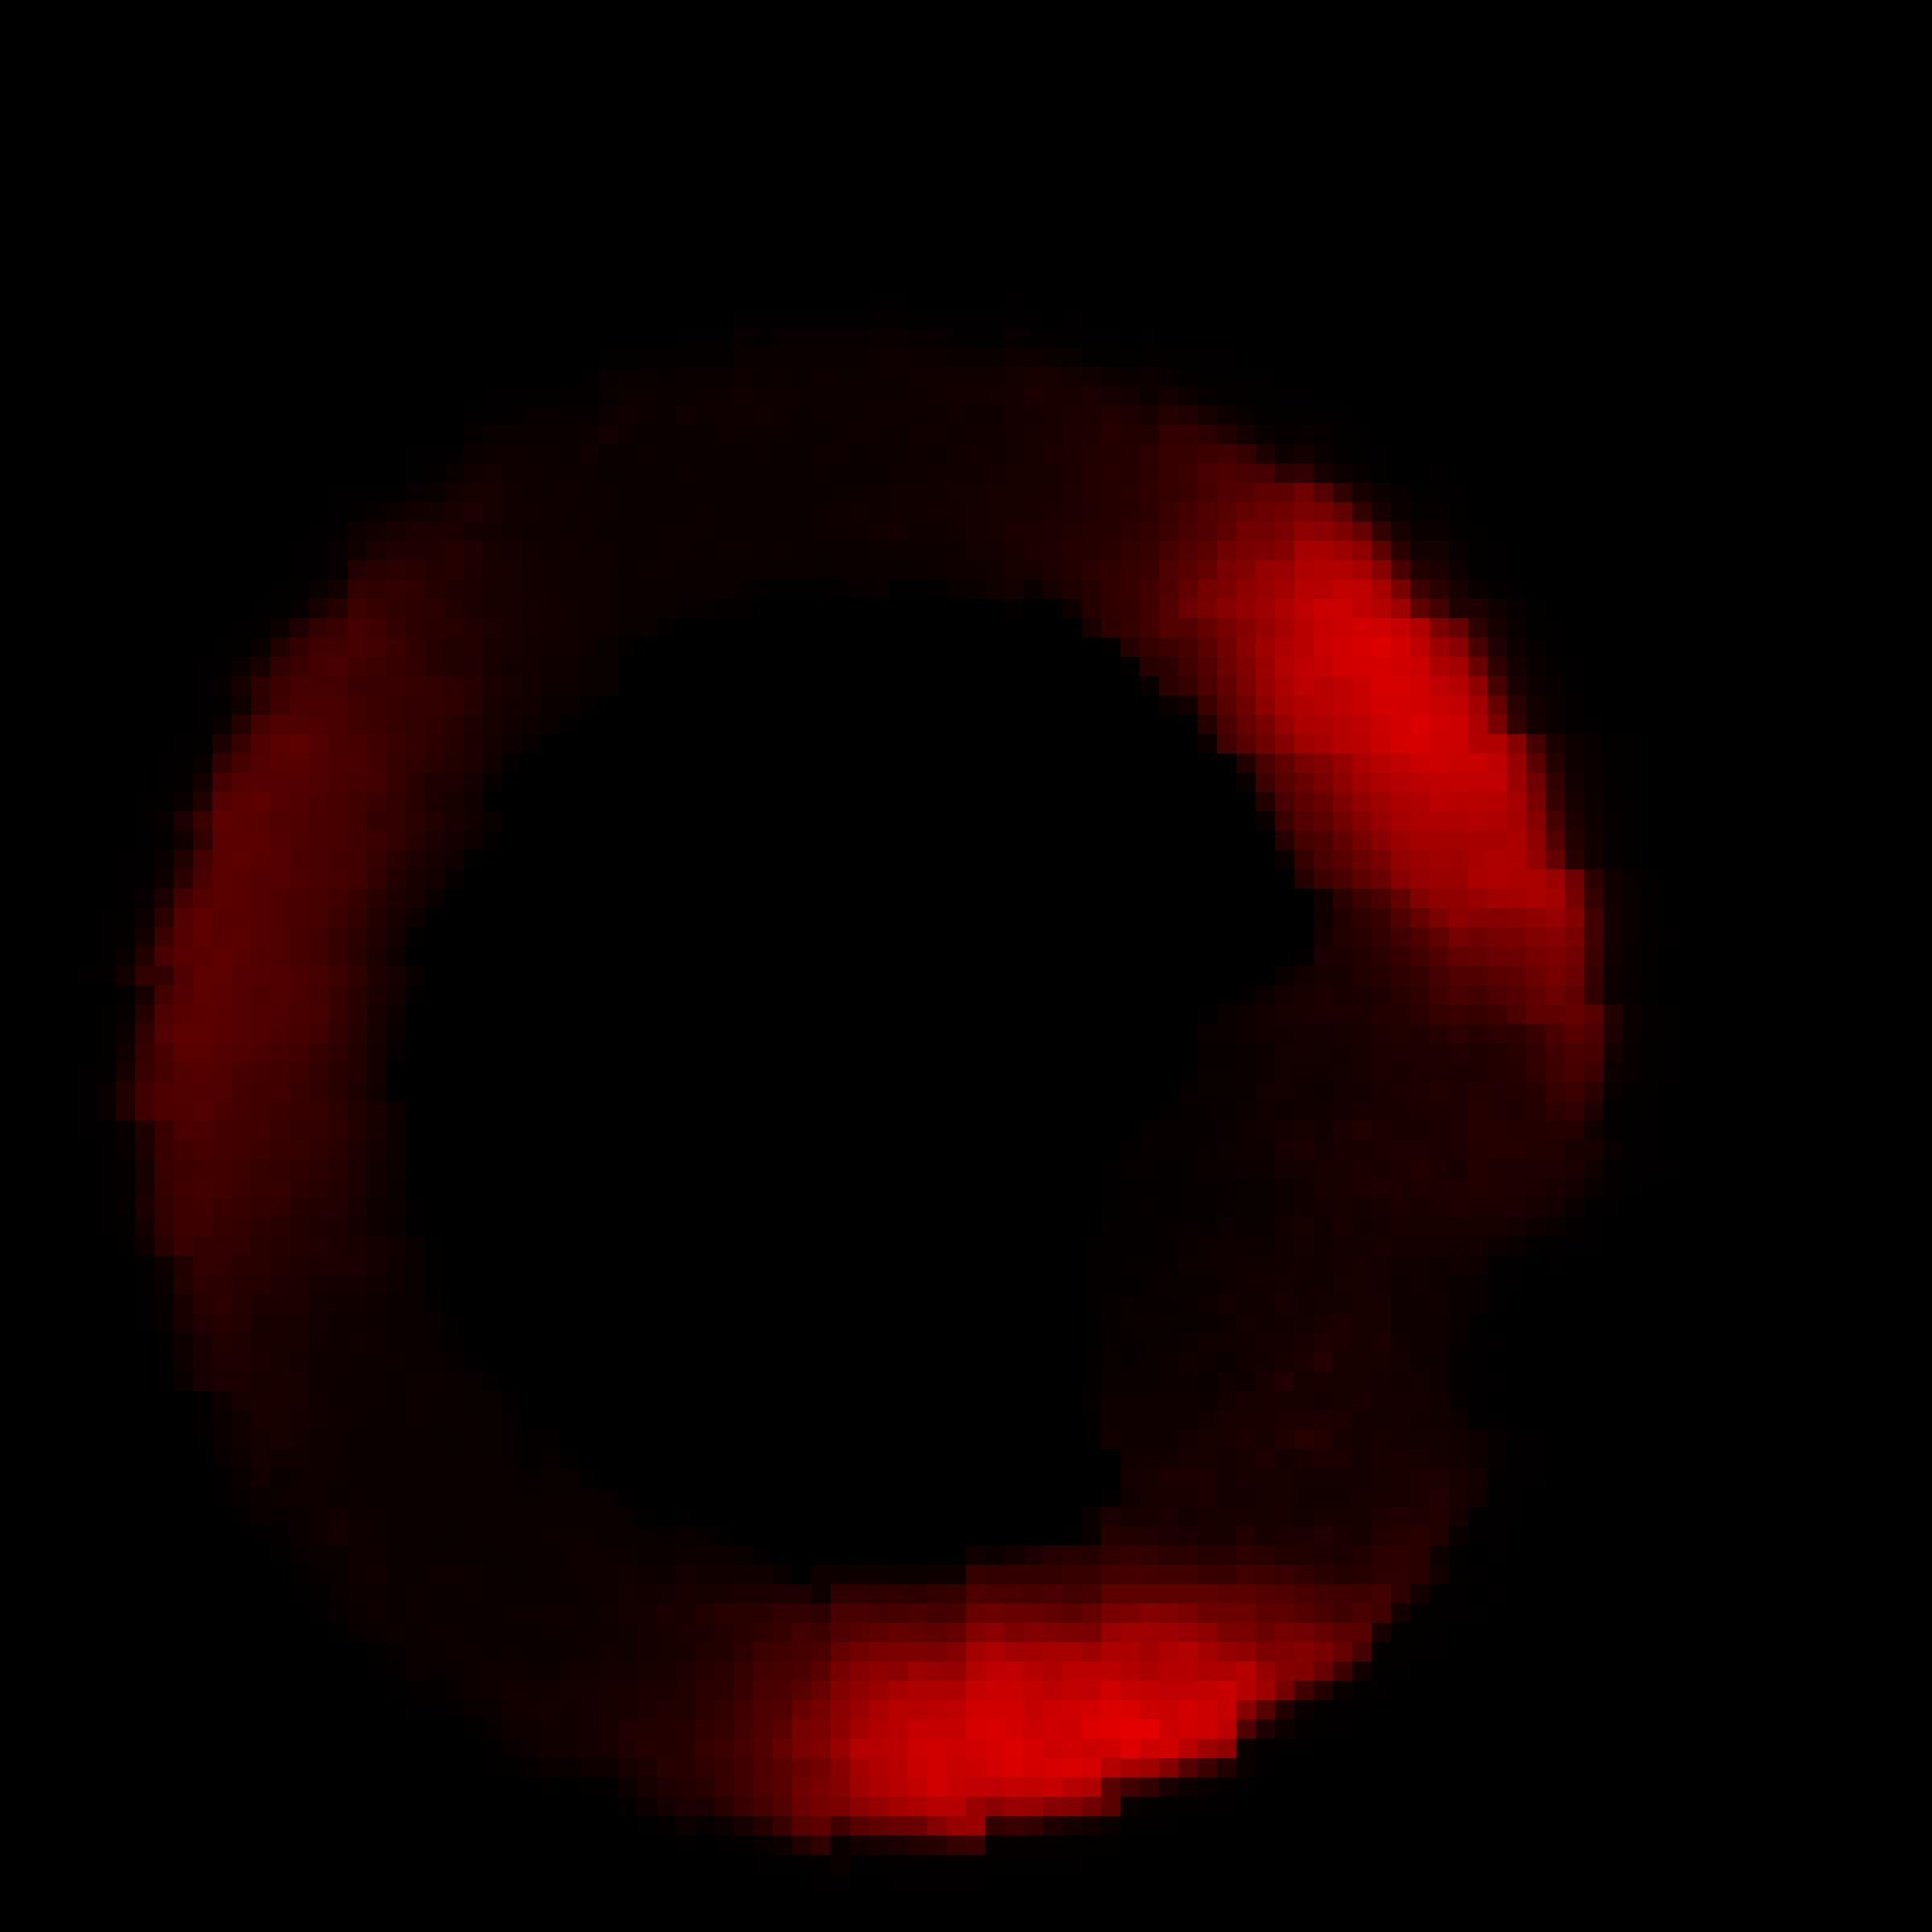
\includegraphics[width=0.1\textwidth]{dpERK_vdm_5}};	    
    	\draw[->] (x1) -- (fig1.north);
    	\draw[->] (x2) -- (fig2.north);
    	\draw[->] (x3) -- (fig3.north);
    	\draw[->] (x4) -- (fig4.north);
    	\draw[->] (x5) -- (fig5.north);
    \end{tikzpicture}
    
\end{frame}

\begin{frame}{Scattering Transform as Image Features}

{\small 
\begin{itemize}
	\item Thus far, we have only used the Euclidean distance as our metric.
	%
	\item Another option is to use {\em features} of the images, and then take distances between these features to use in our DMAPS calculations.
	%
	\item 
	We will use the scattering transform \footcite{bruna2012invariant} as features of our images.
\end{itemize}
\par}
\vspace{-0.15in}
\begin{minipage}{0.55\textwidth}
\begin{block}{{\small Scattering transform is like the Fourier transform \par}}
\centering 
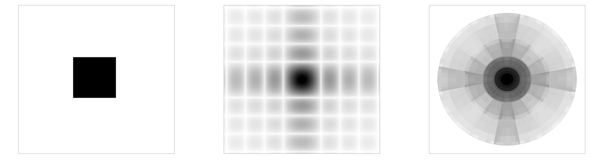
\includegraphics[width=0.75\textwidth]{scat_images/shapeimage_2}\\
{\tiny (Left) $f$ = indicator of a square, (Center) Modulus of the Fourier transform of $f$, (Right) Scattering transform of $f$ \par}
\end{block}

\vspace{-0.1in}
\begin{block}{{\small Scattering transform is robust to deformations \par}}
\centering
\animategraphics[width=0.8\textwidth,autoplay,loop]{5}{scat_images/animate_}{0}{3}\\
{\tiny (Left) $f$ = Gabor atom of varying frequency and direction, (Center) Modulus of the Fourier transform of $f$, (Right) Scattering transform of $f$ \par}
\end{block}

\end{minipage}
\hfill
\begin{minipage}{0.4\textwidth}
\begin{block}{{\small Scattering transform can discriminate higher-order structures \par}}
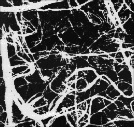
\includegraphics[height=0.15\textheight]{scat_images/texture8-1}
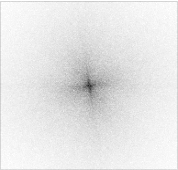
\includegraphics[height=0.15\textheight]{scat_images/texture8-f1}
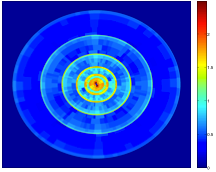
\includegraphics[height=0.15\textheight]{scat_images/shapeimage_3}

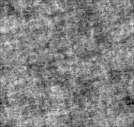
\includegraphics[height=0.15\textheight]{scat_images/texture8-eq}
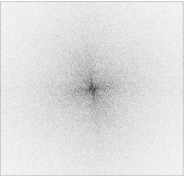
\includegraphics[height=0.15\textheight]{scat_images/texture8-f1eq}
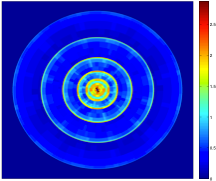
\includegraphics[height=0.15\textheight]{scat_images/shapeimage_4}\\
{\tiny (Left) $X_1, X_2$ = Two realizations of stationary textures. $X_2$ is obtained by equalizing random white noise according to the spectrum of $X_1$. (Center) Power spectrum of $X_1$, $X_2$. (Right) Scattering transform of $X_1$, $X_2$. High order scattering coefficients discriminate between the Gaussian process $X_2$ and the non-Gaussian $X_1$. \par}
\end{block}

\end{minipage}

\end{frame}

\begin{frame}{Ordering of Two-Dimensional Images}

	{\small 
	\begin{itemize}
		\item We compute the scattering transform coefficients for the images.
		\item We use the Euclidean distance {\em between the scattering transform coefficents} in our DMAPS calculation.
	\end{itemize}
    \par}
    
    \centering
    \begin{tikzpicture}
    	\node[anchor=south west] (image) {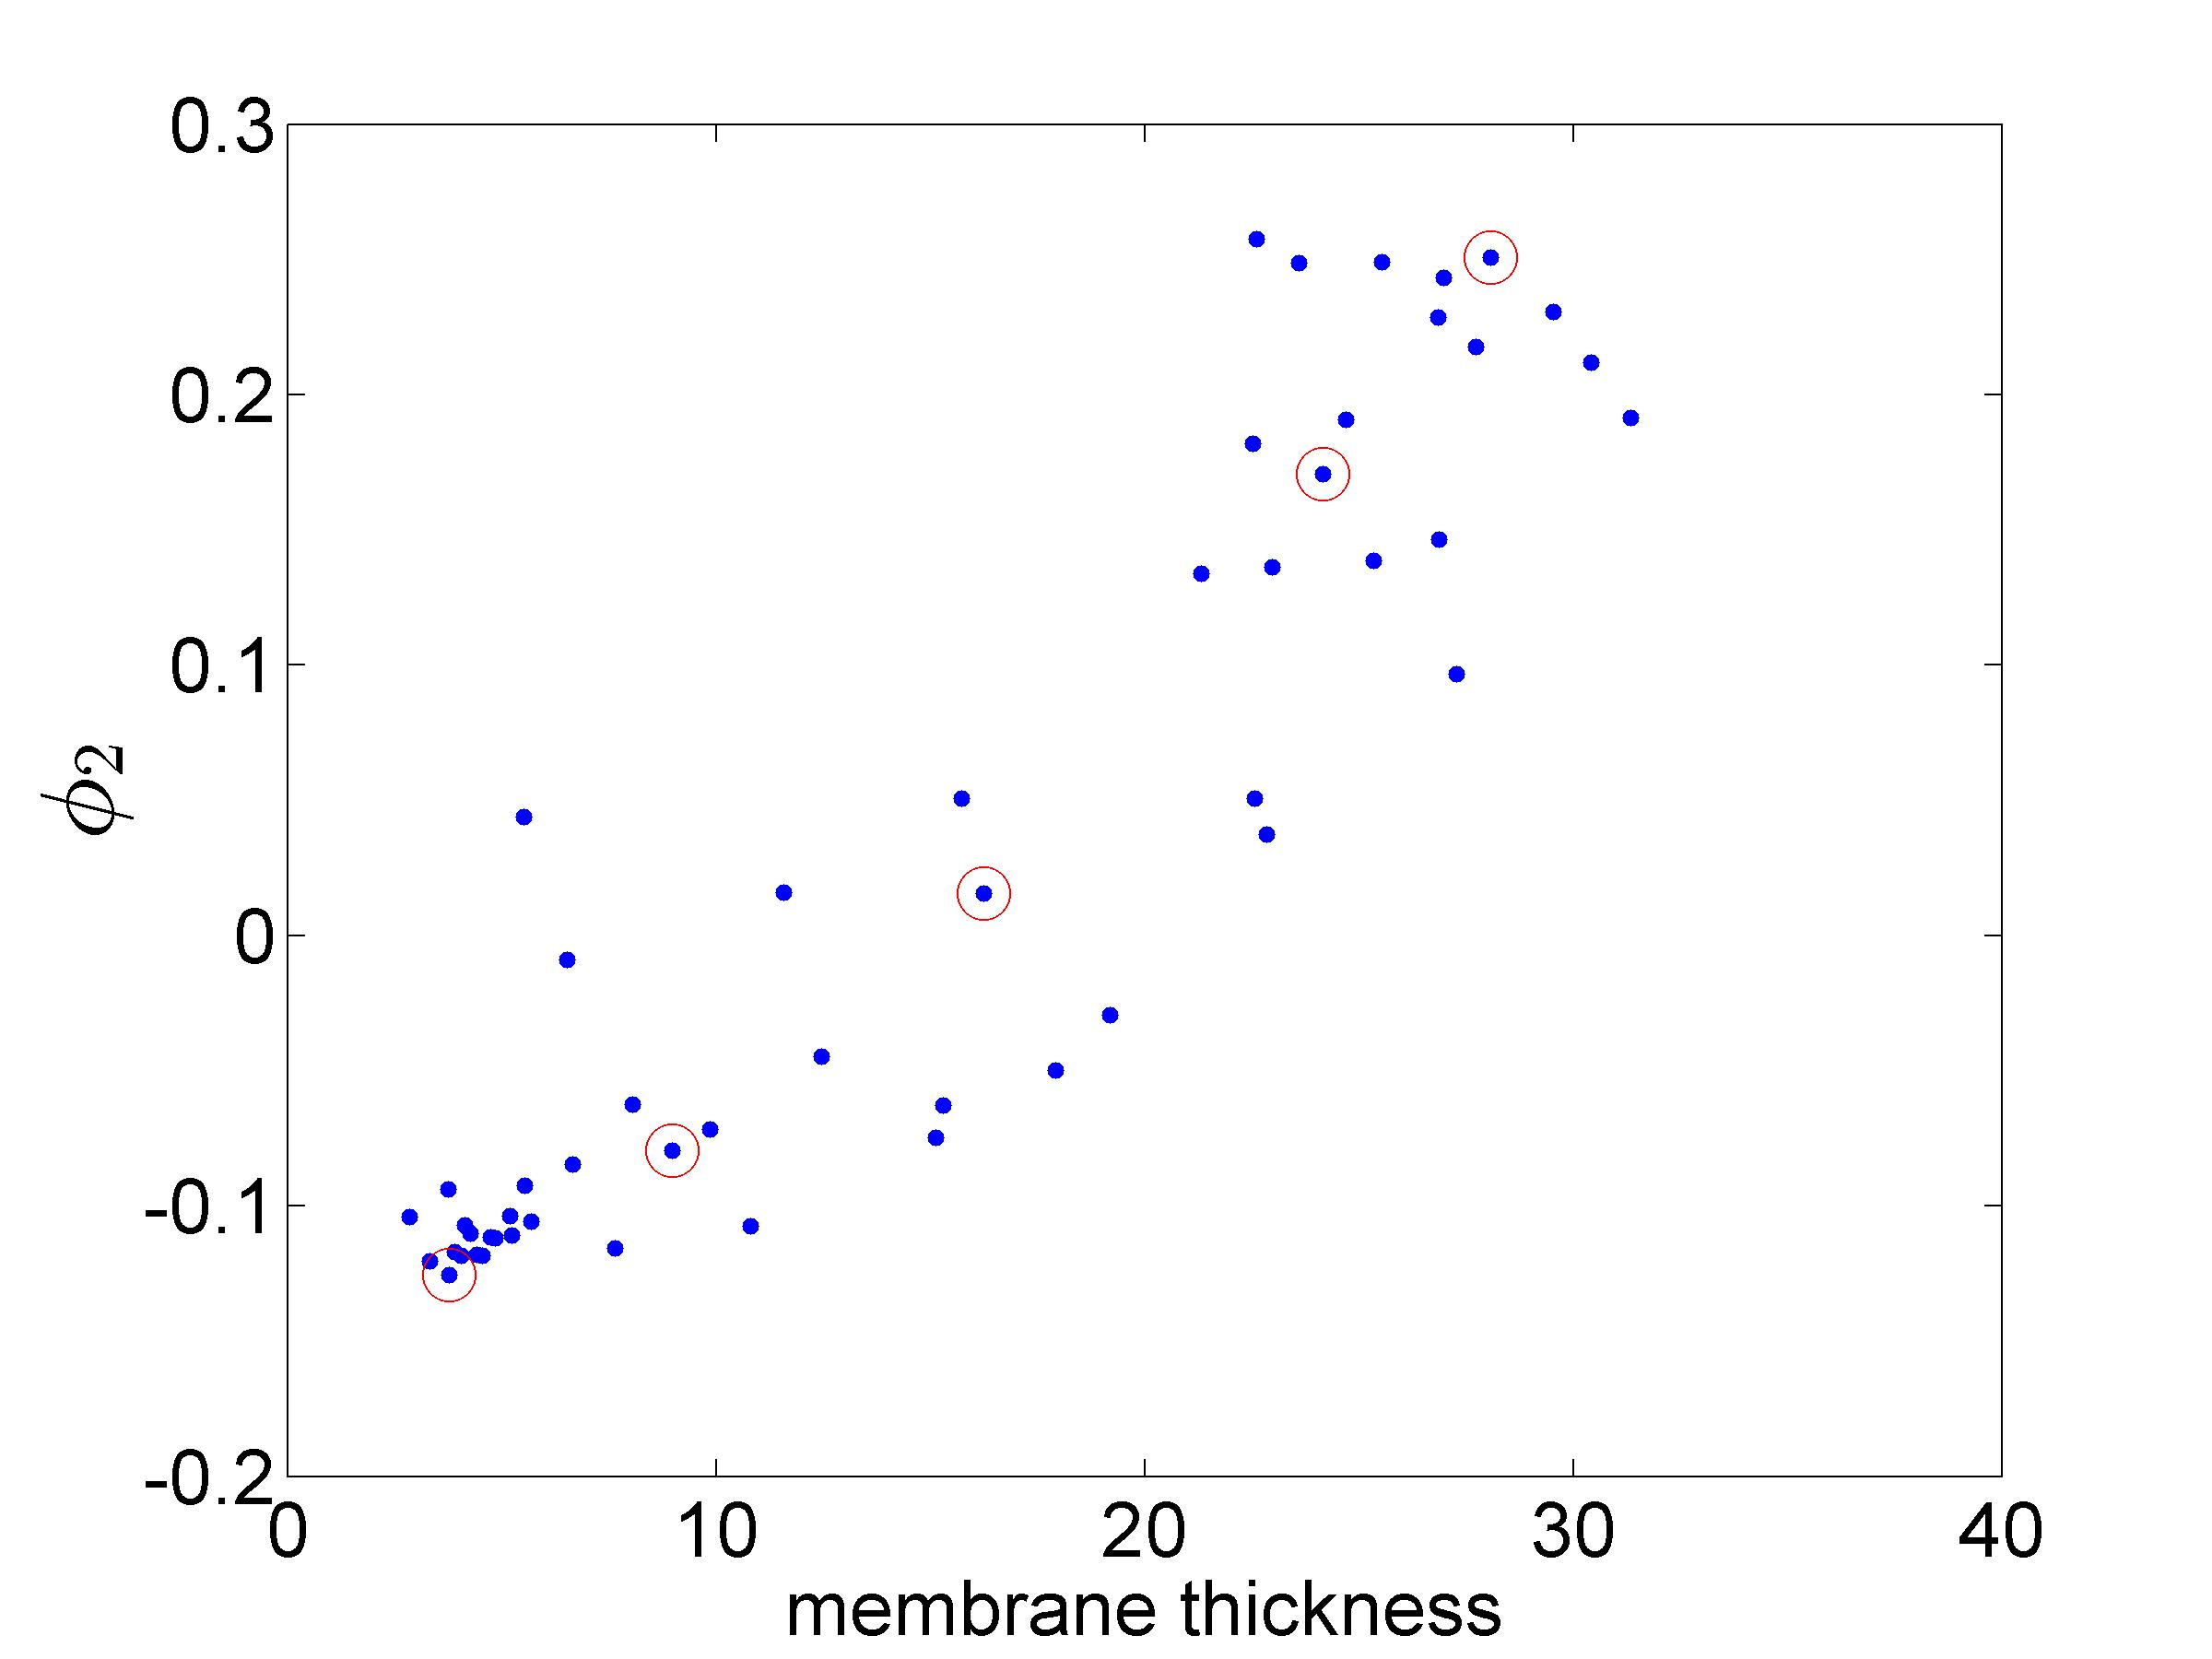
\includegraphics[width=0.45\textwidth]{DMAPS_scat_time_corr2}};
    	\begin{scope}[x={(image.south east)},y={(image.north west)}]
    	%\draw[help lines,xstep=.05,ystep=.05] (0,0) grid (1,1);
    	\node(x1) at (0.23,0.24) {};
    	\node(x2) at (0.32,0.32) {};
    	\node(x3) at (0.45,0.49) {};
    	\node(x4) at (0.59,0.72) {};
    	\node(x5) at (0.66,0.85) {};
    	\end{scope}
    	\node[below=0.2in of image](fig3) {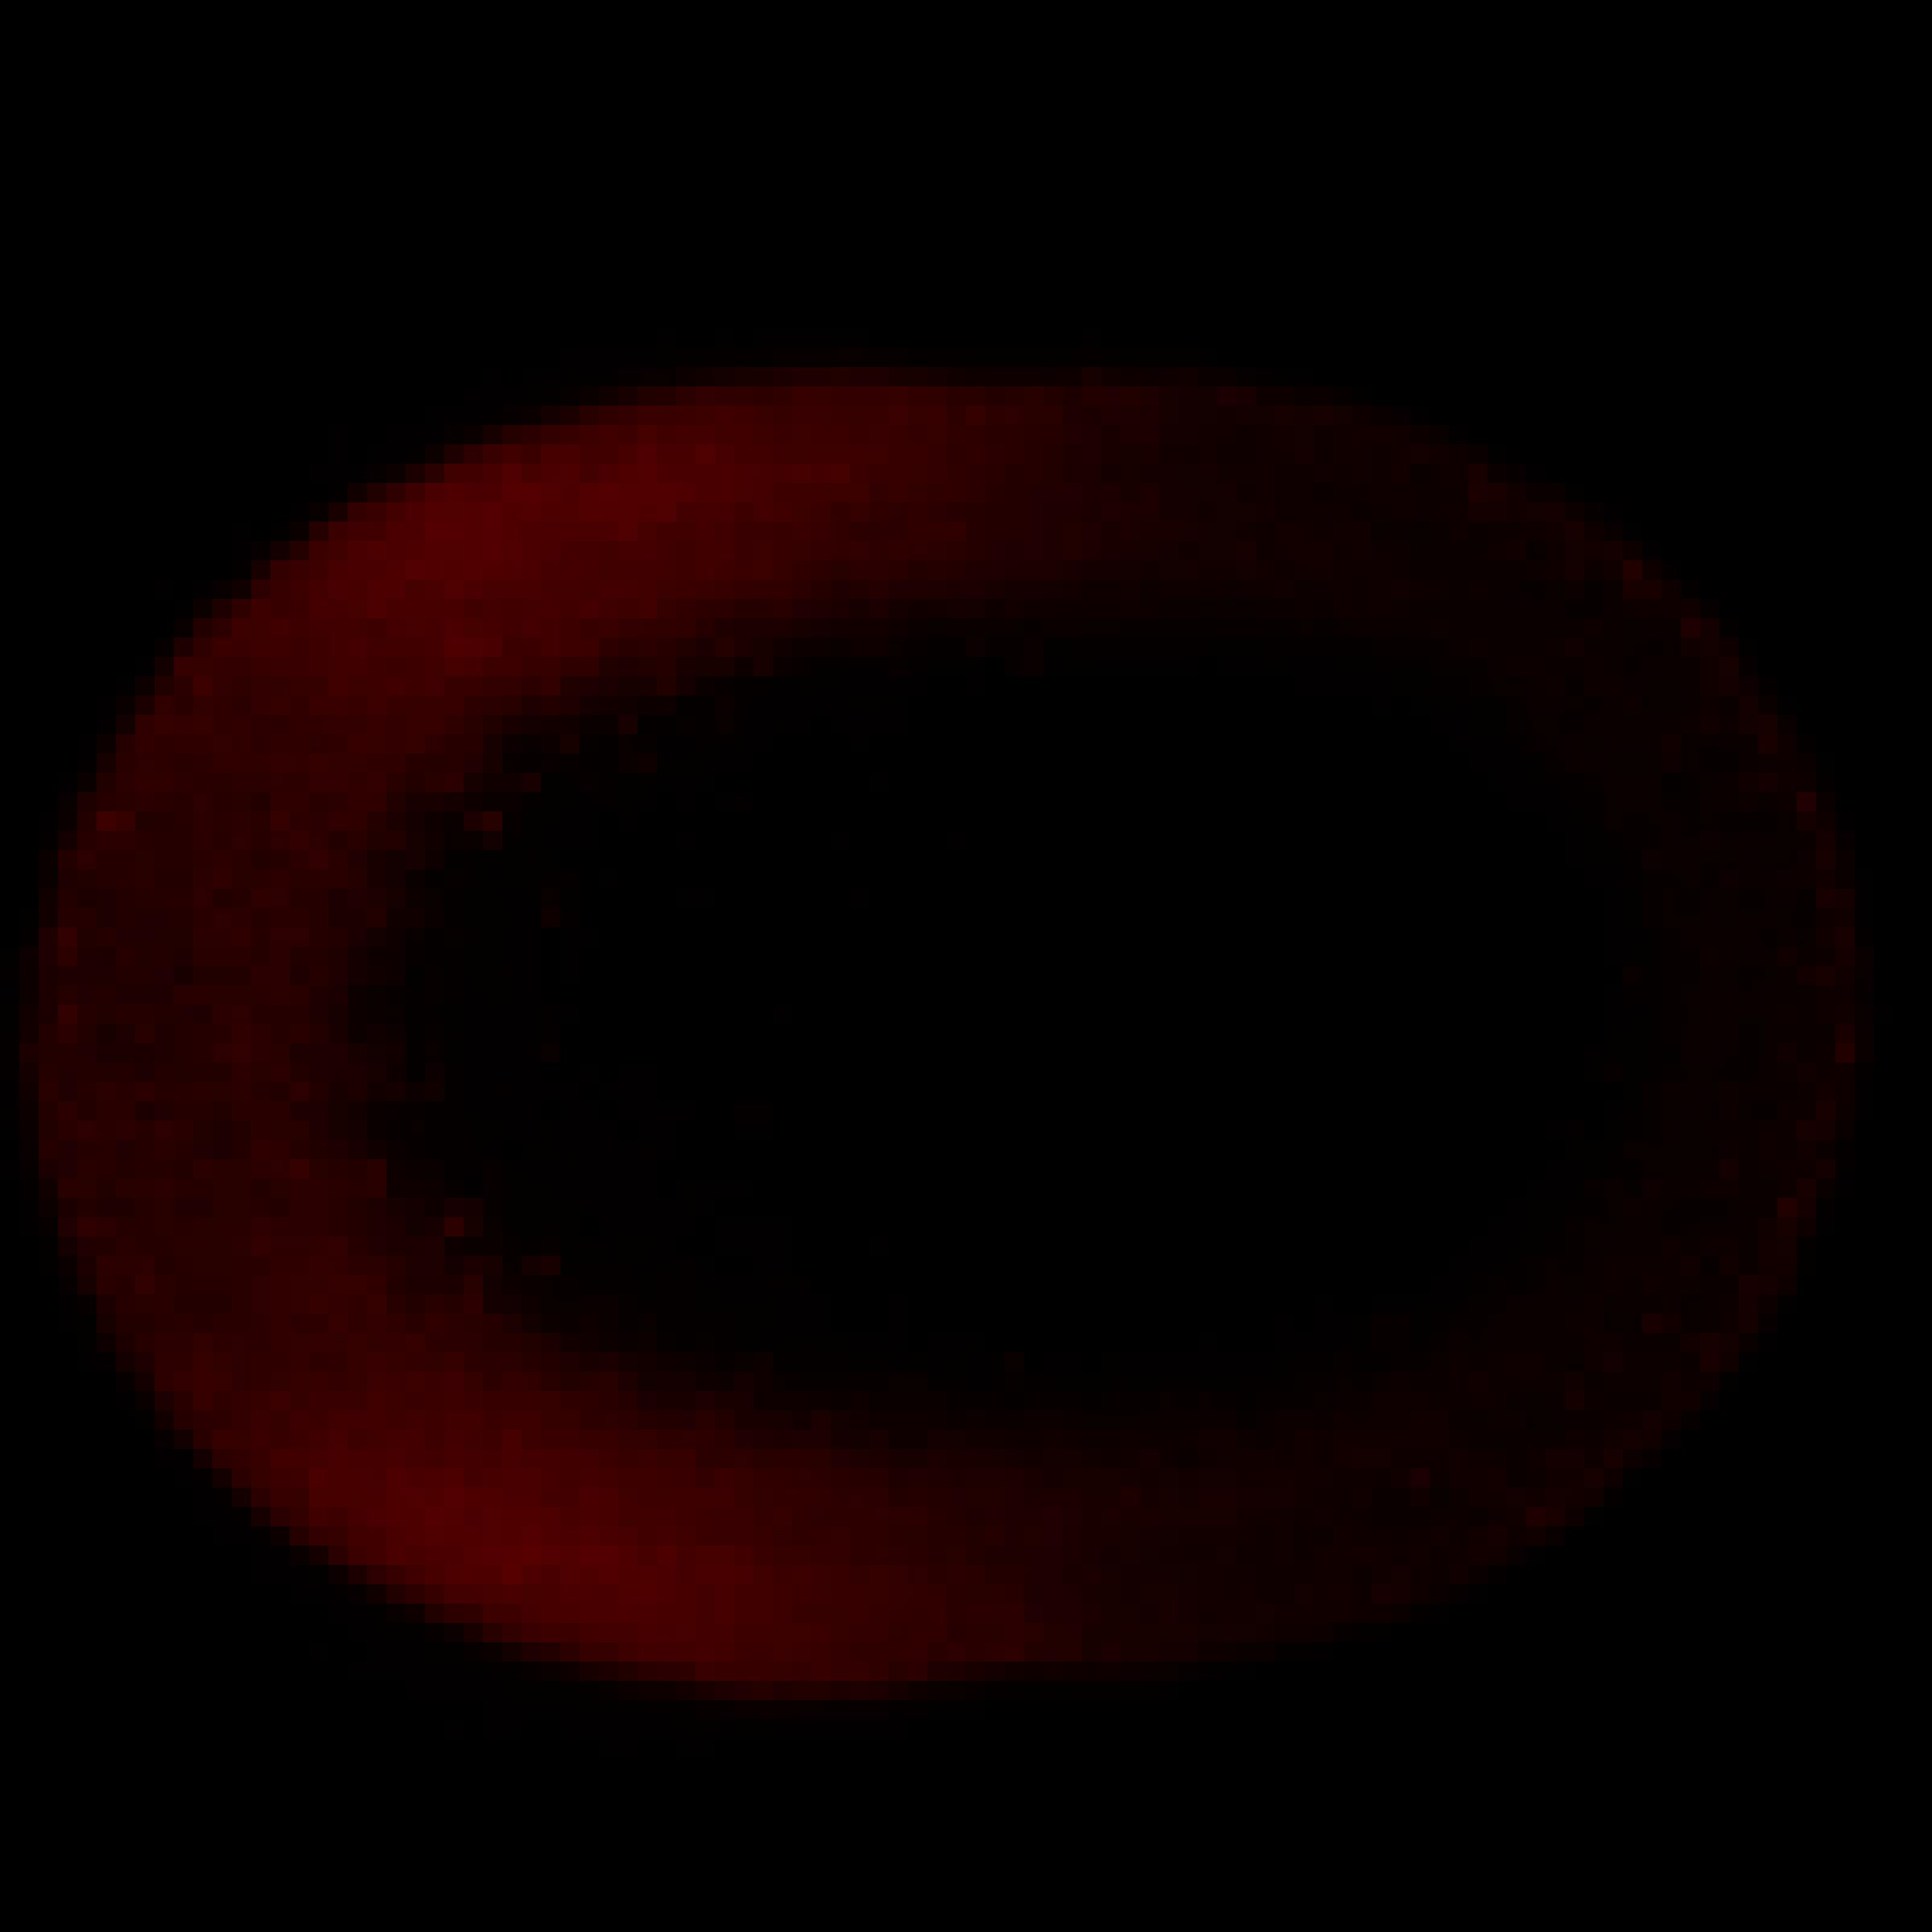
\includegraphics[width=0.07\textwidth]{dpERK_scat_3}};		
    	\node[left=0.1in of fig3](fig2) {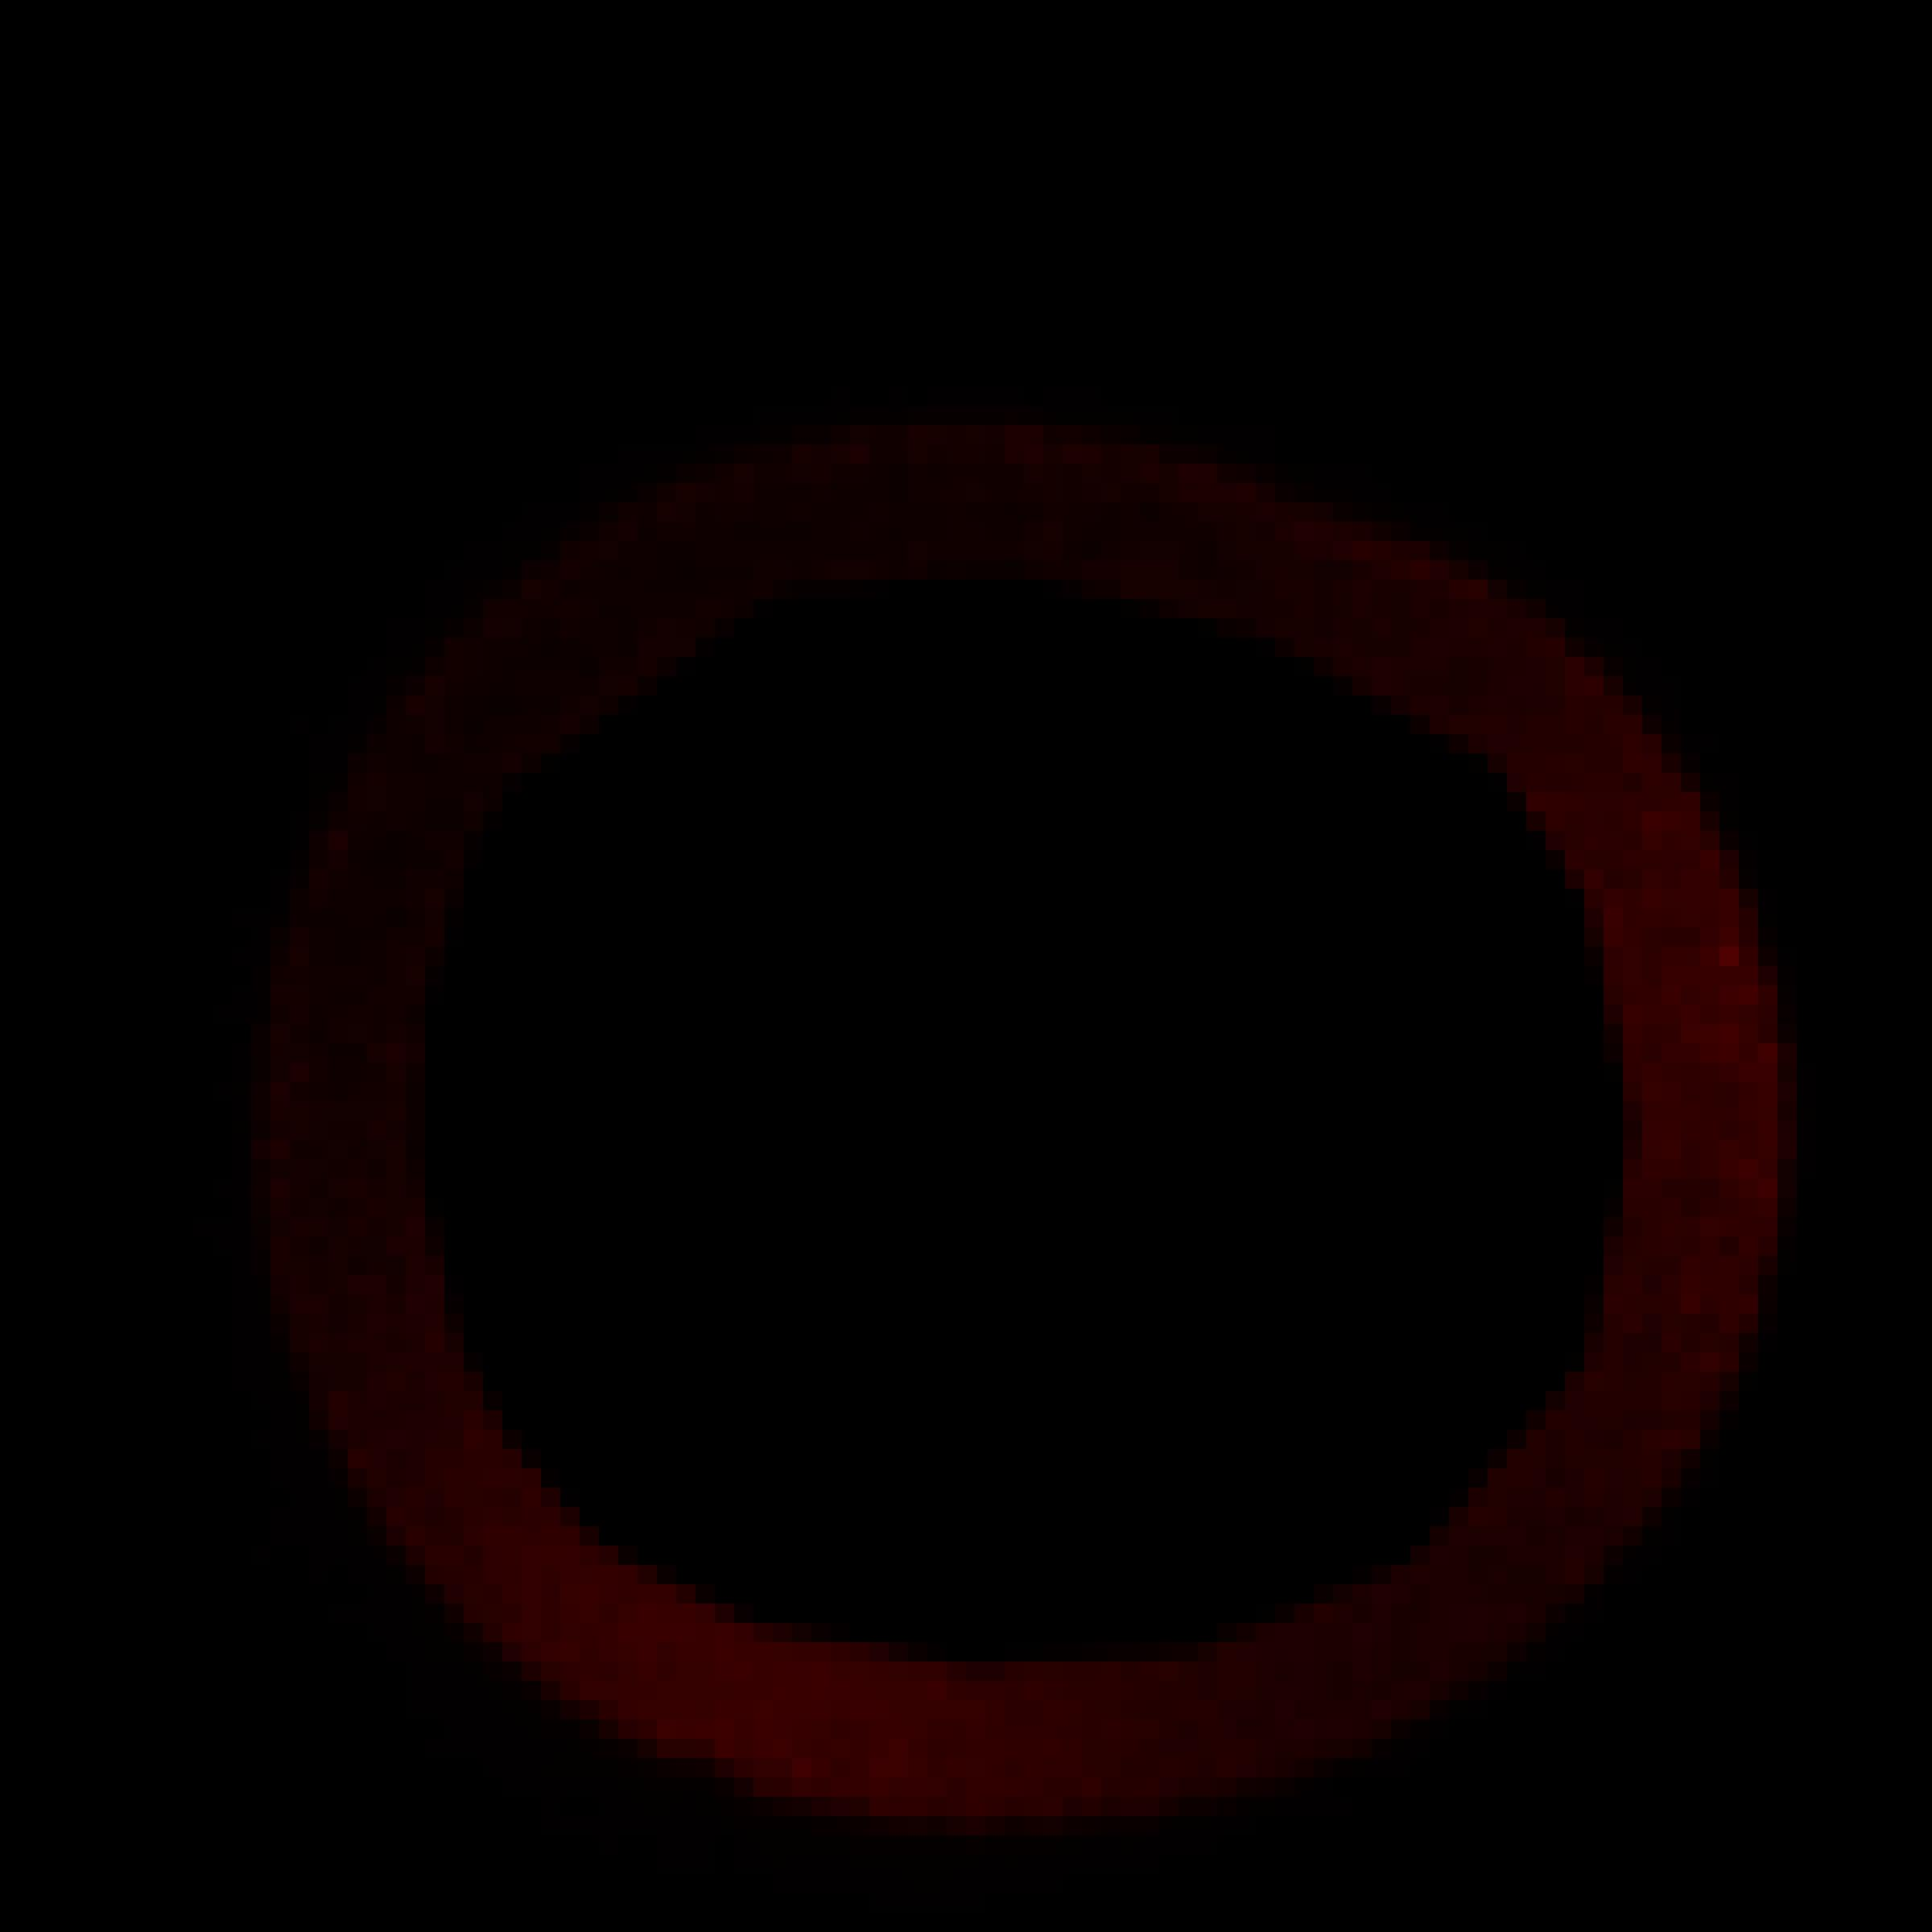
\includegraphics[width=0.07\textwidth]{dpERK_scat_2}};
    	\node[left=0.1in of fig2](fig1) {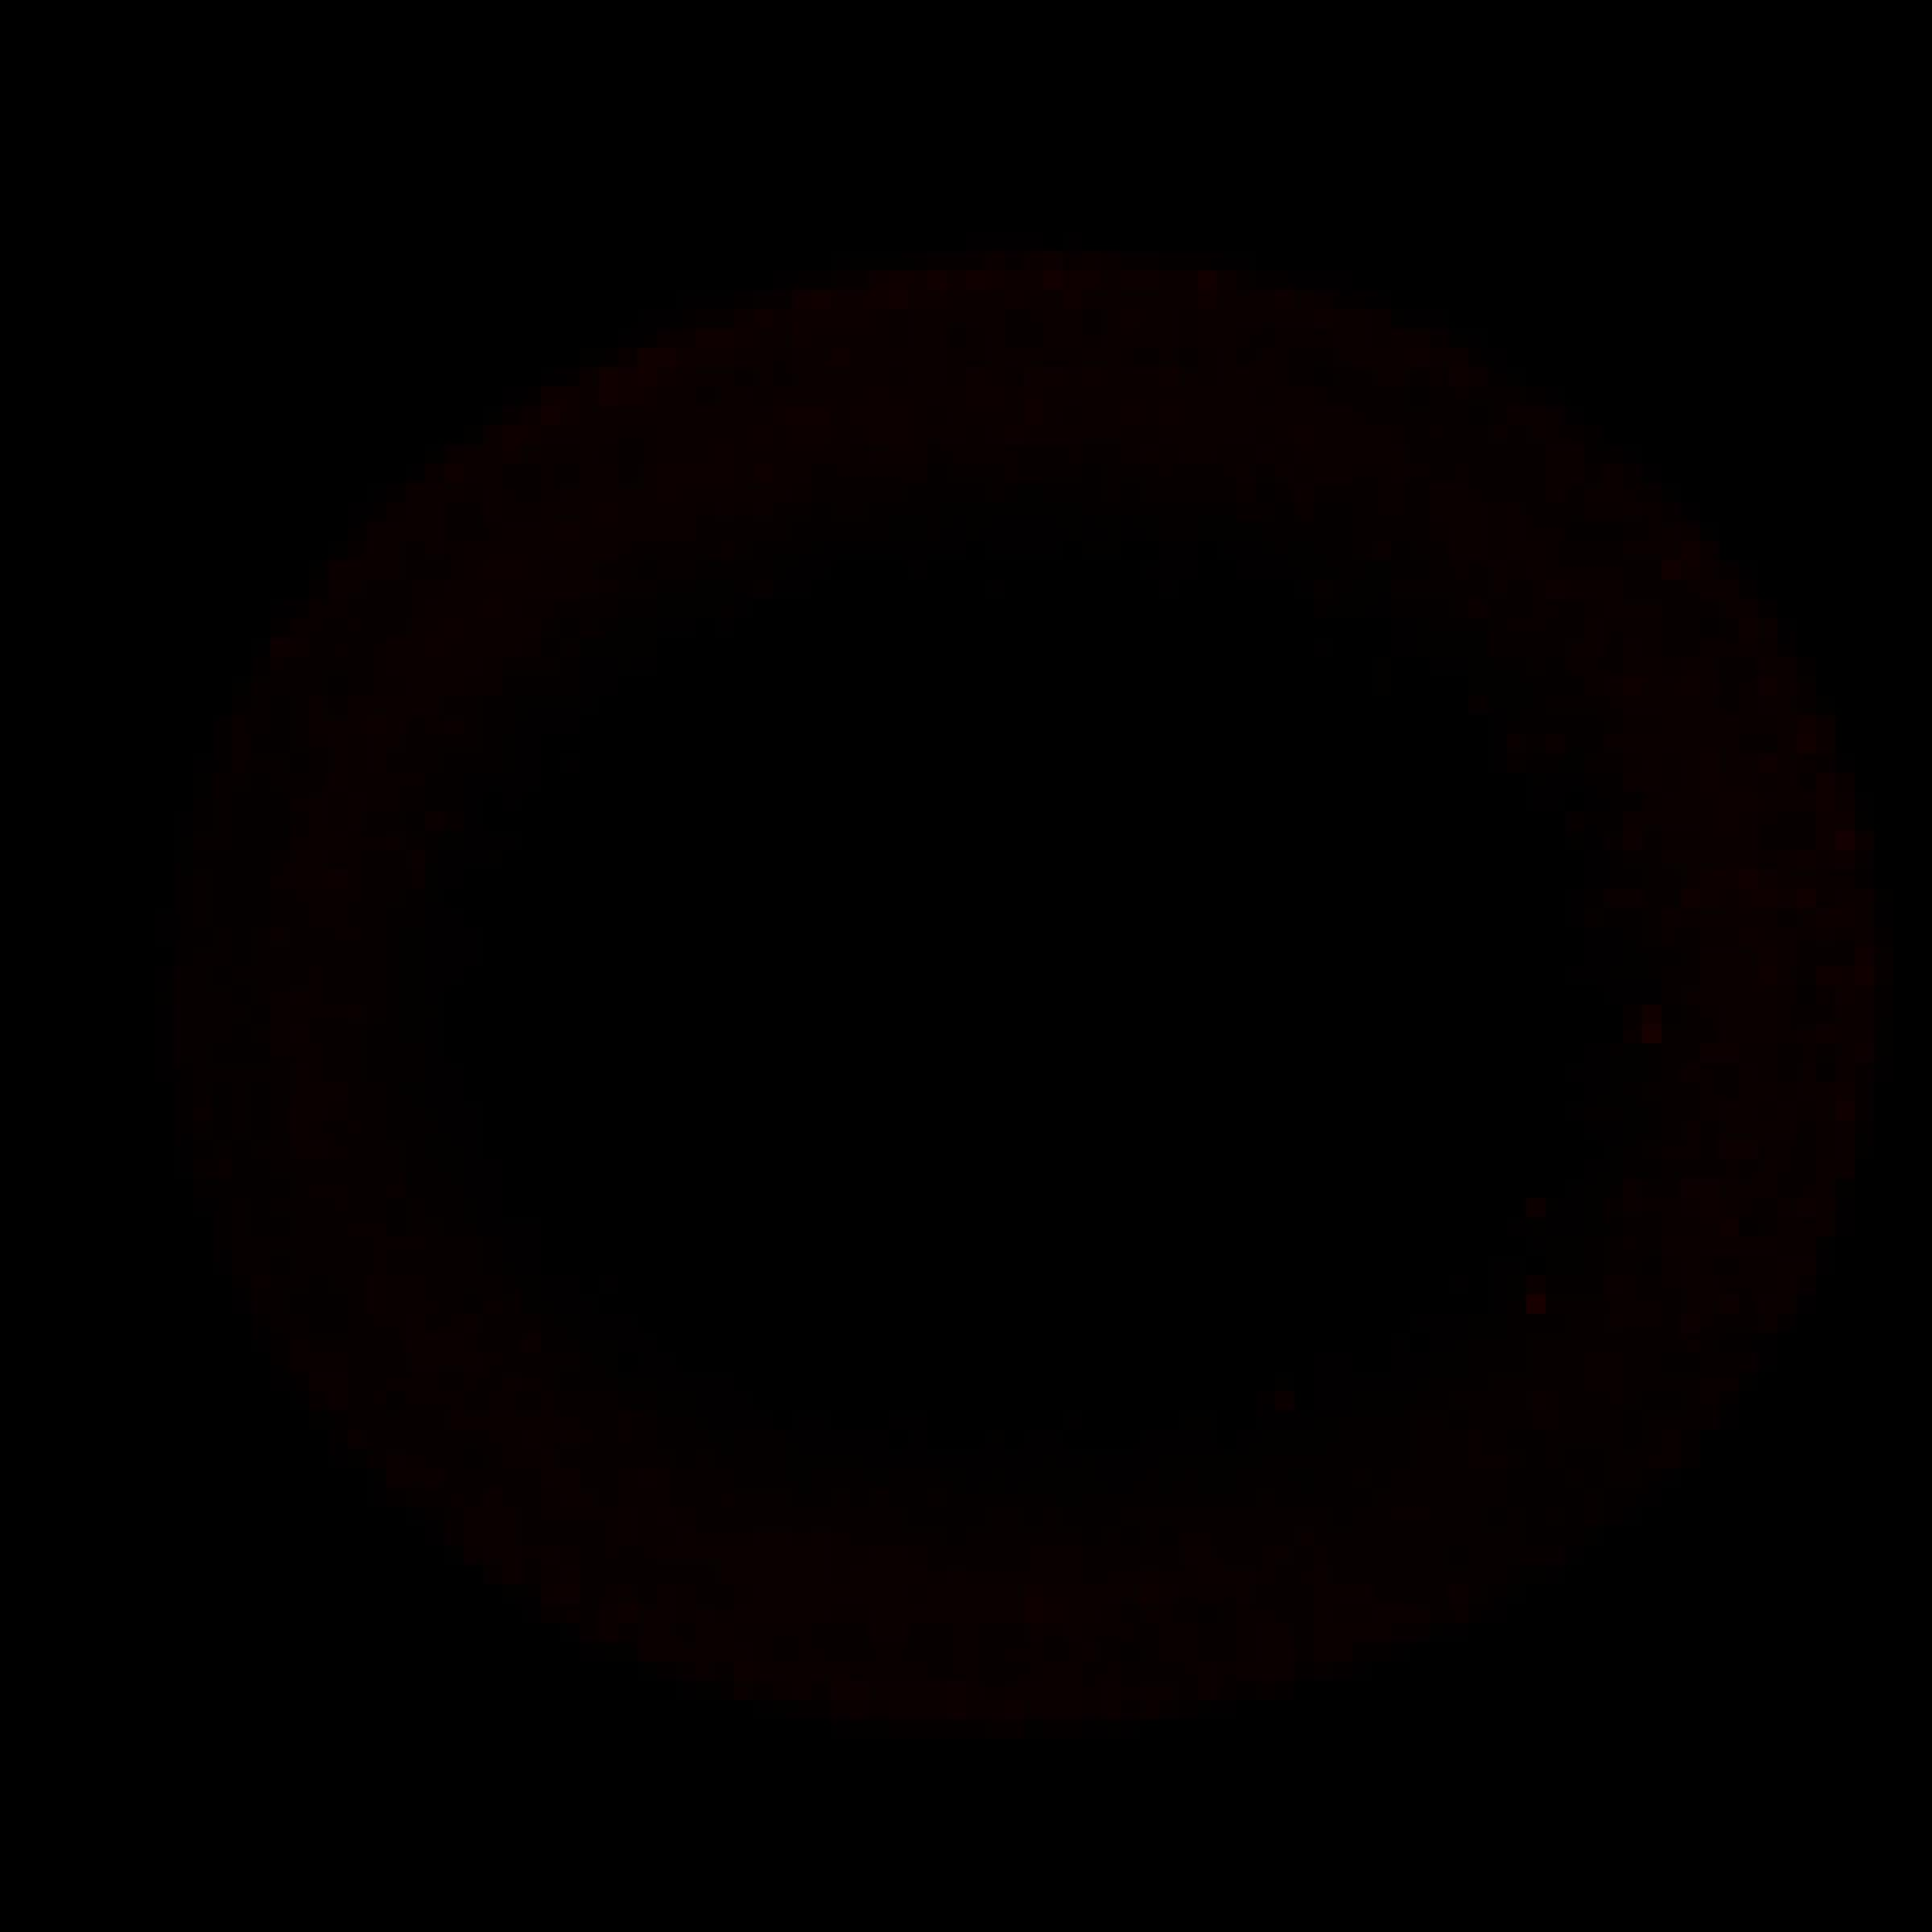
\includegraphics[width=0.07\textwidth]{dpERK_scat_1}};	
    	\node[right=0.1in of fig3](fig4) {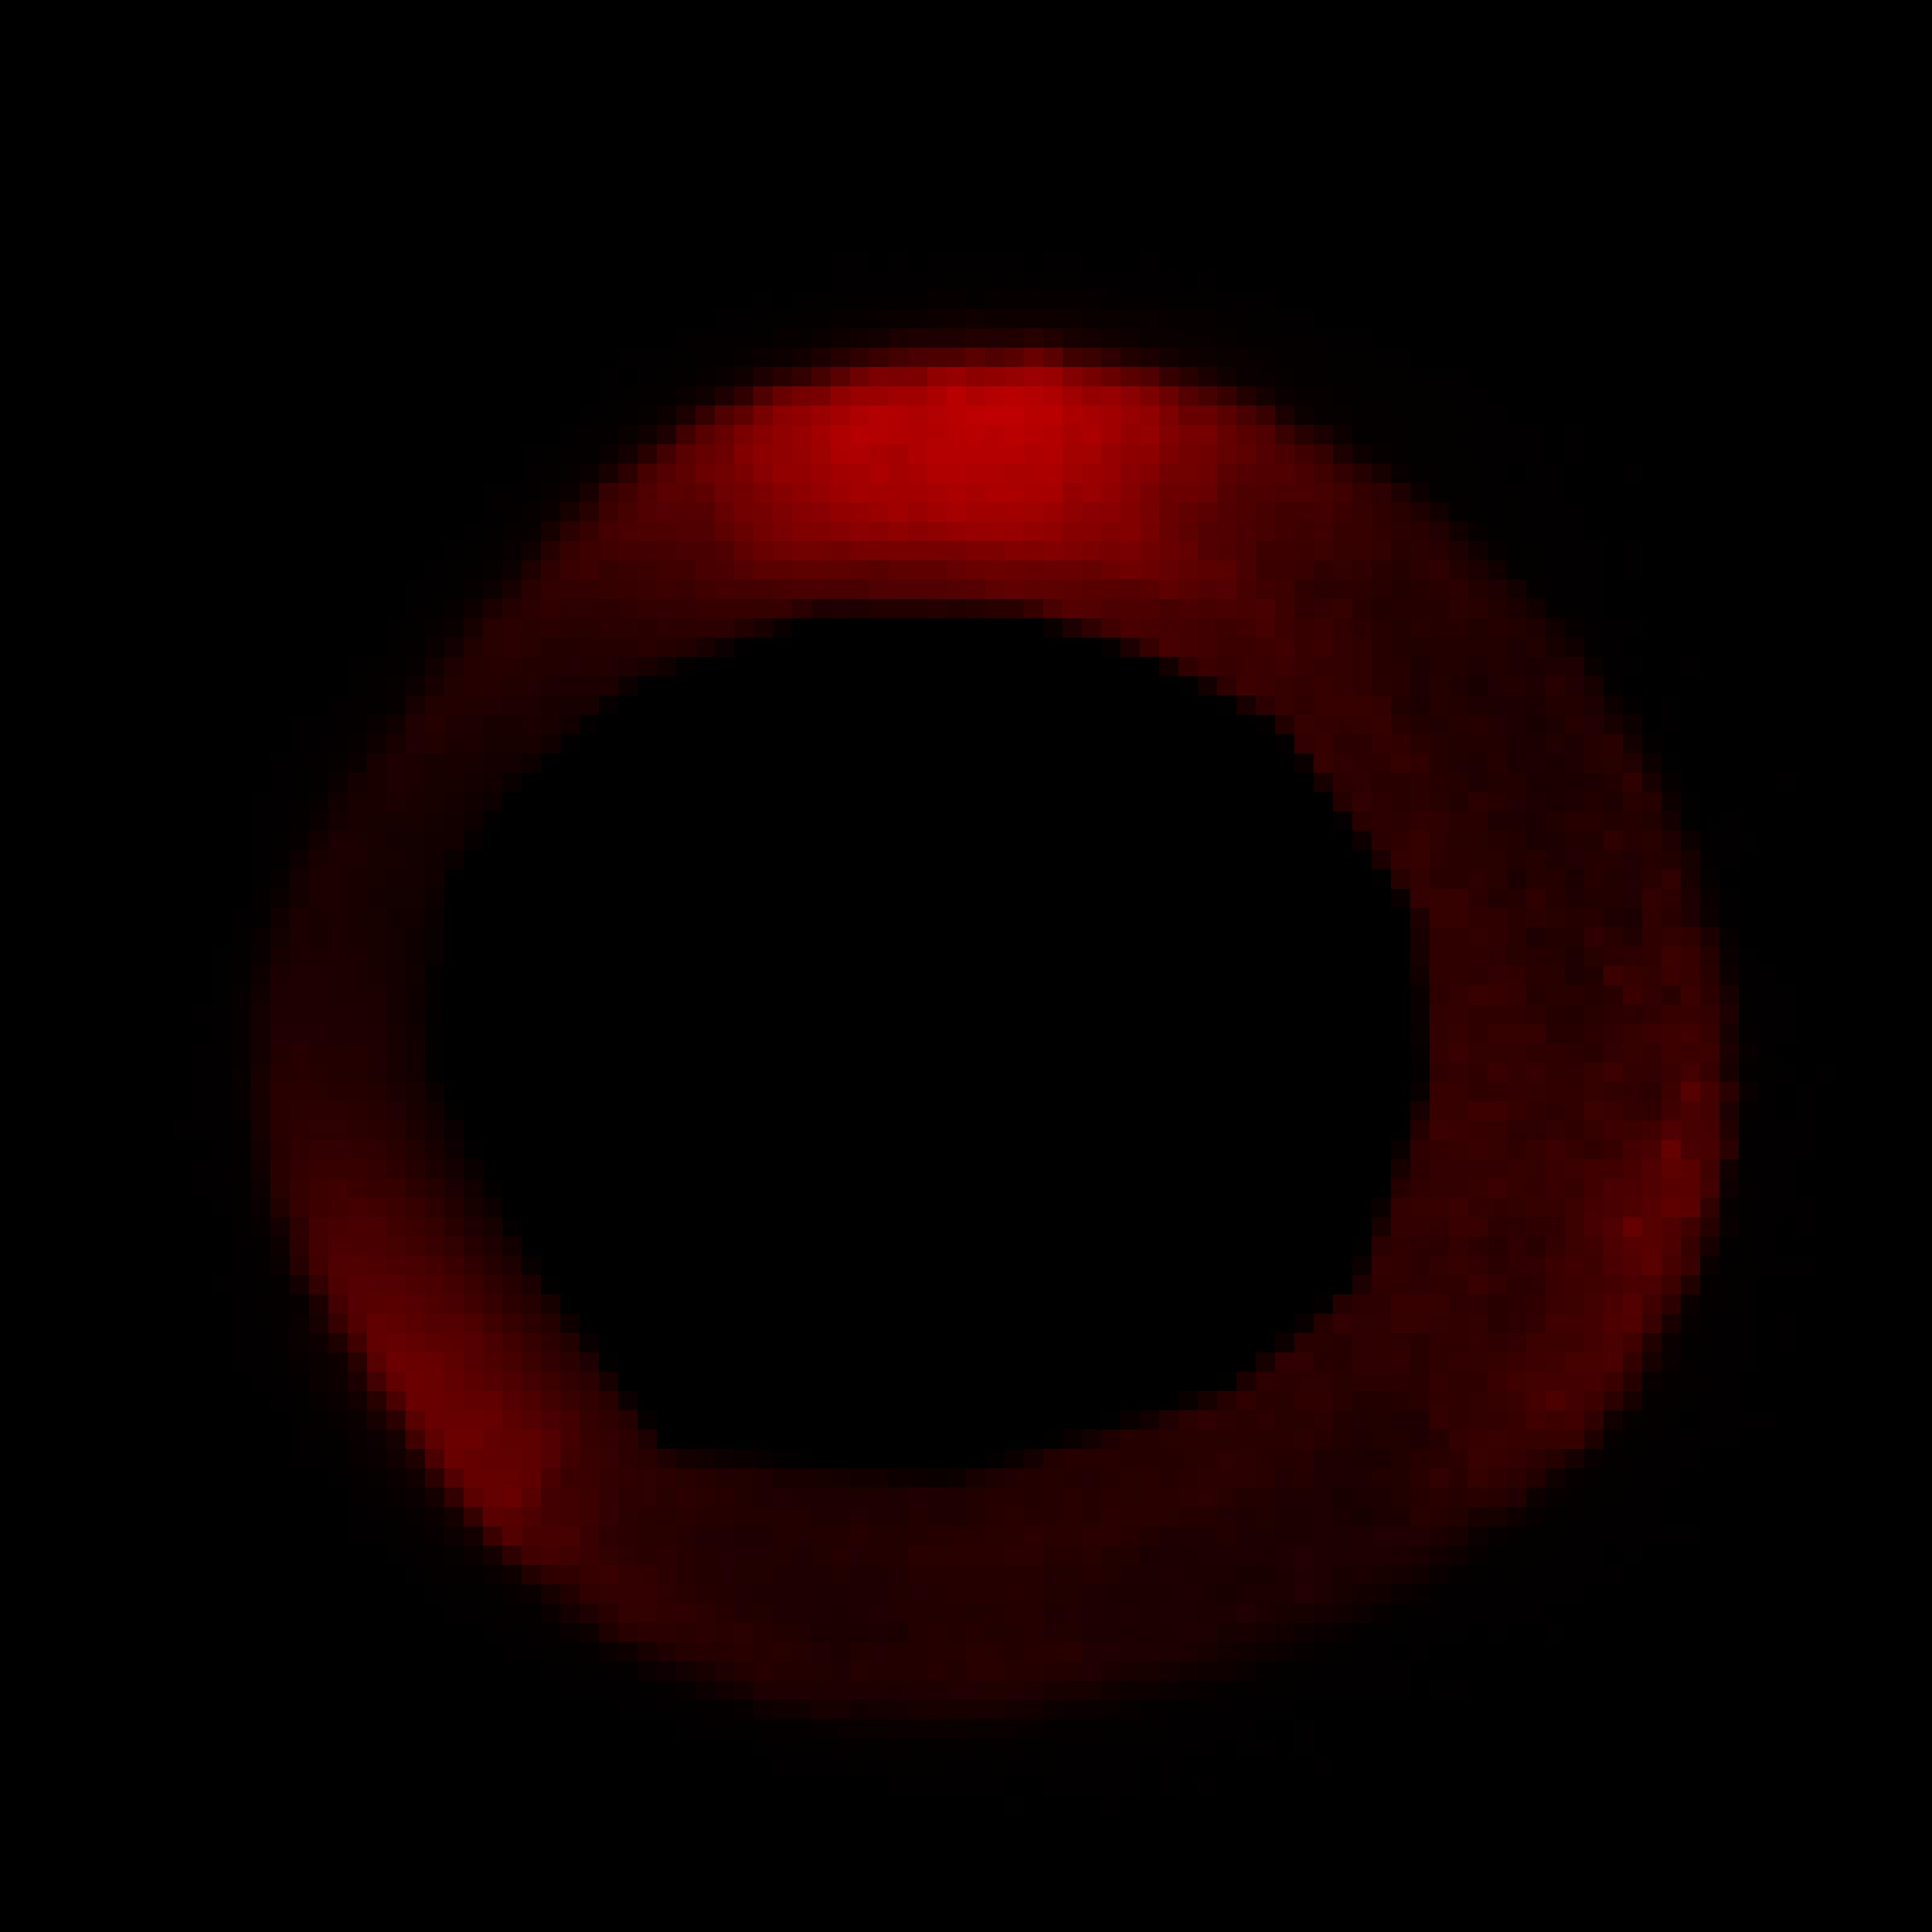
\includegraphics[width=0.07\textwidth]{dpERK_scat_4}};					
    	\node[right=0.1in of fig4](fig5) {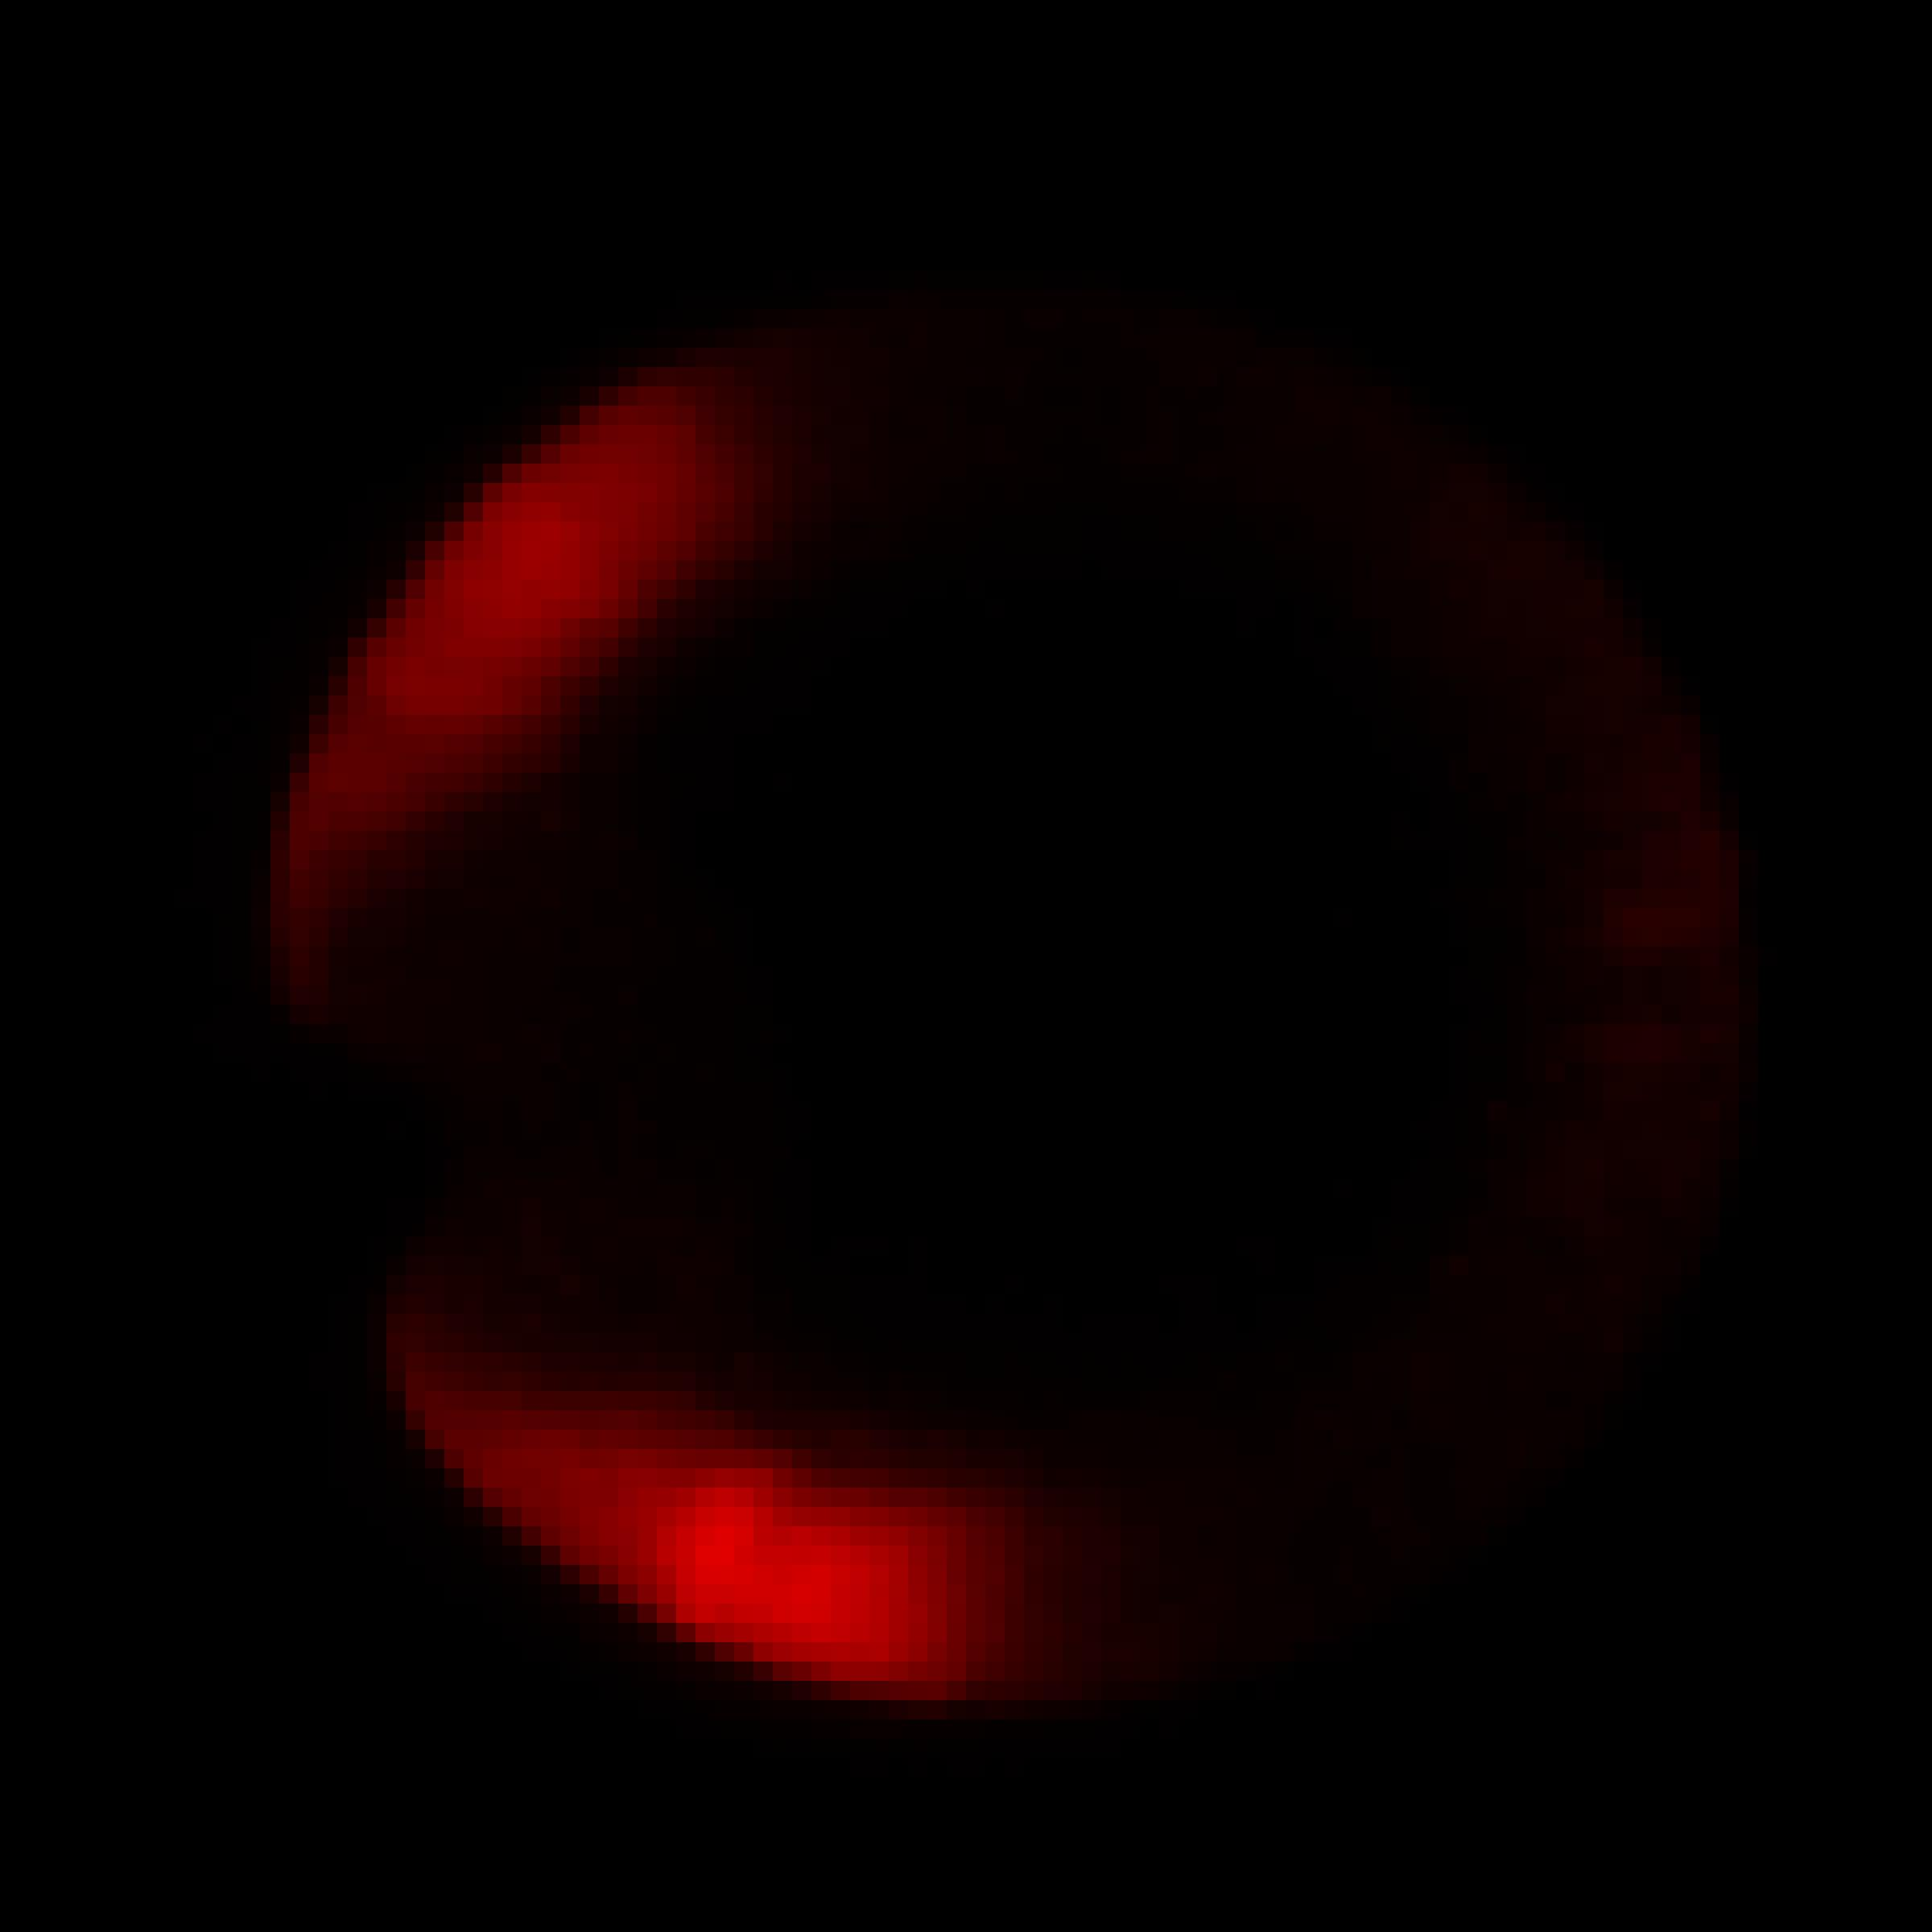
\includegraphics[width=0.07\textwidth]{dpERK_scat_5}};	    
    	\draw[->] (x1) -- (fig1.north);
    	\draw[->] (x2) -- (fig2.north);
    	\draw[->] (x3) -- (fig3.north);
    	\draw[->] (x4) -- (fig4.north);
    	\draw[->] (x5) -- (fig5.north);
    \end{tikzpicture}
	
	The first DMAPS coordinate is well-correlated with the membrane thickness.
    
\end{frame}

    
    

    